\begin{figure}[h]
  \centering
\begin{minipage}{120pt}
   \fontsize{7pt}{8pt}\selectfont
   \texttt{\textbf{Point} p, q, r, s} \\
   \texttt{\textbf{Segment} a := \{p, q\}} \\
   \texttt{\textbf{Segment} b := \{p, r\}} \\
   \texttt{\textbf{Point} m := \textbf{Midpoint}(a)} \\
   \texttt{\textbf{Angle} theta := $\angle$(q, p, r)} \\
   \texttt{\textbf{Triangle} t := \{p, r, s\}} \\
   \texttt{\textbf{Ray} w := \textbf{Bisector}(theta)} \\
   \texttt{\textbf{Ray} h := \textbf{PerpendicularBisector}(a)} \\
\end{minipage}%
\hspace{0pt}%
\begin{minipage}{340pt}
   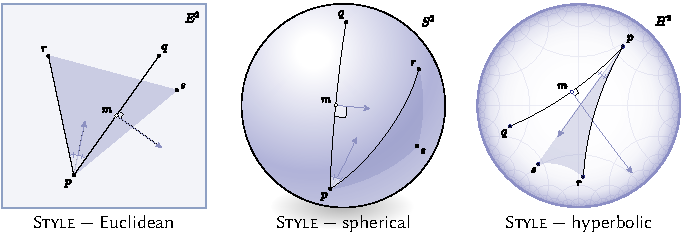
\includegraphics{assets/penrose/teaser.pdf}
\end{minipage}
   \caption{\Penrose{} is a framework for specifying how mathematical statements should be interpreted as visual diagrams.  A clean separation between abstract mathematical objects and their visual representation provides new capabilities beyond existing code- or GUI-based tools.  Here, for instance, the same set of statements (left) is given three different visual interpretations (right), via Euclidean, spherical, and hyperbolic geometry.
   \label{fig:penrose-teaser}
   }
\end{figure}

Informed by the results from the interview study (\cref{chp:interviews}), colleagues and I have developed \Penrose, a language-based diagramming platform~\cite{penrose}. The core \Penrose system addresses \textbf{representation salience} and \textbf{vocabulary correspondence}: it has first-class support for creating and reusing visual representations and translates familiar math-like notation into one or more possible visual representations. To accomplish this, \Penrose decomposes the concerns of diagramming into two domain-specific languages (DSLs) with distinct purposes: \colorbox[HTML]{E7F3E7}{\Substance} contains the mathematical content in math notation. \colorbox[HTML]{DDDEED}{\Style} explicitly specifies mappings from mathematical objects to visual icons. In contrast to tools that specify diagrams via direct manipulation or low-level graphics programming, \Penrose{} enables rapid creation and exploration of diagrams that faithfully preserve the underlying mathematical meaning.  We demonstrate the effectiveness and generality of the system by showing how it can be used to illustrate a diverse set of concepts from mathematics and computer graphics.

\section{Introduction}
\label{sec:Introduction}

A central goal of this work is to lower the barrier to turning mathematical ideas into effective, high-quality visual diagrams.  In the same way that \TeX\ and \LaTeX\ have democratized mathematical writing by algorithmically codifying best practices of professional typesetters~\cite{Beeton:2016:CMT}, \Penrose{} aims to codify best practices of mathematical illustrators into a format that is reusable and broadly accessible.

Our approach is rooted in the natural separation in mathematics between abstract definitions and concrete representations. In particular, the \Penrose{} system is centered around the specification of a \emph{mapping} from mathematical objects to visual icons (\cref{sec:SystemDesign}).  Such mappings are expressed via domain-specific languages (DSLs) that reflect familiar mathematical notation and can be applied to obtain new capabilities that are difficult to achieve using existing tools (\cref{sec:RelatedSystems}).  A key distinction is that \Penrose{} programs encode a \emph{family} of possible visualizations, rather than one specific diagram.  Hence, effort put into diagramming can easily be reused, modified, and generalized.  This approach has several broad-reaching benefits:

\begin{itemize}
   \item \textbf{Accessibility.} Novice users can generate diagrams by simply typing mathematical statements in familiar notation, leveraging the efforts of more expert package developers.
   \item \textbf{Separation of content and presentation.} The ability to easily swap out different visual representations helps deepen understanding by illustrating the same mathematical concepts from many different visual perspectives.
   \item \textbf{Evolution of collections.} Existing collections of diagrams can easily be improved and modified to meet the needs of a target platform, \eg{} desktop vs. mobile, different printing processes, or different language localizations.
   \item \textbf{Large-scale generation.} It becomes easy to generate large collections of illustrations to explore an idea, or to accompany, say, randomly-generated homework exercises.
   %\item \textbf{Interactive exploration.} Diagrams preserve a given set of relationships \emph{by construction}, and can hence be manipulated without violating the intended mathematical meaning.
\end{itemize}

Beyond describing the implementation of \Penrose{}, the purpose of this chapter is to explore the general challenge of designing systems for diagram generation. We hence start with a discussion of goals and trade-offs that inform our system design (\cref{sec:SystemDesign}). Readers may also find it helpful to periodically refer to the more detailed but purely descriptive account of the system given in \cref{sec:LanguageFramework} and \cref{sec:LayoutEngine}.

\section{System Design}
\label{sec:SystemDesign}


Our aim is to build a system for converting abstract mathematical ideas into visual diagrams.  Choices about system design are guided by several specific goals, many of which are supported by interviews presented in \cref{chp:interviews}:
\begin{enumerate}
   \item Mathematical objects should be expressed in a familiar way.\refstepcounter{goalcounter}\label{gol:FamiliarNotation} % Later we say: what could be better than mathematical notation?
   \item The system should not be limited to a fixed set of domains.\refstepcounter{goalcounter}\label{gol:NoFixedDomains} % Many new domains in mathematics will undoubtedly be discovered in the coming years.
   \item It should be possible to apply many different visualizations to the same mathematical content.\refstepcounter{goalcounter}\label{gol:ManyViz} % Because there are often many different ways to visually represent a given mathematical idea, i
   \item There should be no inherent limit to visual sophistication.\refstepcounter{goalcounter}\label{gol:sophistication}  % The system should allow use of ``best in class'' graphical algorithms to generate diagrams.
   \item It should be fast enough to facilitate an iterative workflow.\refstepcounter{goalcounter}\label{gol:FastEnough}  % Overall we aim for performance commensurate with other document or presentation creation tools.
   \item Effort spent on diagramming should be generalizable and reusable.\refstepcounter{goalcounter}\label{gol:Reuse}
\end{enumerate}

To achieve these goals, we take inspiration from the way diagrams are often drawn by hand.  In many domains of mathematics, each type of object is informally associated with a standard \emph{visual icon}.  For instance, points are small dots, vectors are little arrows, \etc{}  To produce a diagram, symbols are systematically translated into icons; a diagrammer then works to arrange these icons on the page in a coherent way.  We formalize this process so that diagrams can be generated computationally, rather than by hand.  Specifically,

\begin{figure}[t]
   \centering
   \begin{minipage}[c]{.35\linewidth}
       \caption{High-level pipeline: a compiler translates mathematical statements and a chosen visual representation into a constrained optimization problem.  This problem is then solved numerically to produce one or more diagrams.\label{fig:HighLevelPipeline}}
   \end{minipage}\hfill
   \begin{minipage}[c]{.60\linewidth}
       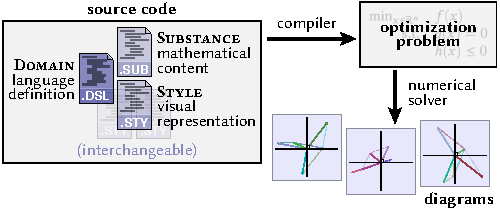
\includegraphics[width=\linewidth]{assets/penrose/HighLevelPipeline.pdf}
   \end{minipage}\hfill
   \vspace{-\baselineskip}
\end{figure}


\vspace{.5\baselineskip}\begin{mdframed}
The two organizing principles of \Penrose{} are:
   \begin{enumerate}[label=(\roman*)]
      \item to \textbf{specify} diagrams via a mapping from mathematical objects to visual icons, and
      \item to \textbf{synthesize} diagrams by solving an associated constrained optimization problem.
   \end{enumerate}
\end{mdframed}\vspace{.5\baselineskip}


Just as the occupant of Searle's ``Chinese room'' does not actually understand a foreign language~\cite{Cole:2014:CRA}, a system designed this way need not perform deep reasoning about mathematics---it simply does a translation.  We hence do not expect our system to solve all challenges of diagramming. Users are still responsible for, say,
\begin{itemize}
   \item choosing meaningful notation for a mathematical domain,
   \item inventing a useful visual representation of that domain, and
   \item ensuring that diagrams correctly communicate meaning.
\end{itemize}

\setlength{\columnsep}{1em}
\setlength{\intextsep}{0em}
\begin{wrapfigure}{r}{0.4\linewidth}
% \begin{figure}
% {128pt}
\begin{minipage}{60pt}
\begin{lstlisting}[language=Sub-ST,escapechar=@,numbers=none]
Set A, B
Point p
A $\subset$ B
p $\in$ A
p $\notin$ B
\end{lstlisting}
\end{minipage}\hfill
\begin{minipage}{120pt}
  \centering
  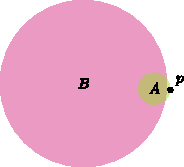
\includegraphics[width=\linewidth]{assets/penrose/sets-inconsistent.pdf}
\end{minipage}
   \vspace{-.5\baselineskip}\caption{An optimization-based approach has myriad benefits.  Here a logically inconsistent program fails gracefully, providing visual intuition for \emph{why} the given statements cannot hold.\label{fig:sets-inconsistent}}
\end{wrapfigure}
% \end{figure}

Likewise, a system cannot be expected to solve hard computational or mathematical problems (\eg the halting problem or Fermat's last theorem) in order to construct diagrams.  Yet despite this shallow level of reasoning, \Penrose{} is able to generate quite sophisticated diagrams.  In fact, even in the absence of such reasoning, na\"{i}ve visualization often provides useful observations (\cref{fig:sets-inconsistent}).

The resulting system effectively models diagram generation as a compilation process, where the compilation target is a constrained optimization problem rather than (say) a binary executable or a static image.  Once compiled, this problem can be used and \emph{reused} to generate visual diagrams; \cref{fig:HighLevelPipeline} illustrates the high-level system flow.  From a programming language point of view, a mapping expressed in this framework defines an \emph{executable visual semantics}. That is, it gives a specific, visual, and computable interpretation to what were previously just abstract logical relationships.

\subsection{Language-Based Specification}
\label{sec:LanguageBasedSpecification}

\begin{figure}
   \centering
   %\includegraphics{assets/penroseRetargeting.pdf}
   \begin{minipage}[c]{.30\linewidth}
   \caption{By specifying diagrams in terms of abstract relationships rather than explicit graphical directives, they are easily adapted to a wide variety of use cases.  Here we use identical \Penrose{} code to generate ray tracing diagrams for several targets (\cref{sec:RayTracing}).  Though the arrangement and number of objects changes in each example, the meaning remains the same.\label{fig:Retargeting}}
  \end{minipage}\hfill
  \begin{minipage}[c]{.6\linewidth}
   \begin{overpic}{assets/penrose/Retargeting.pdf}
      \put(60,15) {\parbox{2in}{
         \texttt{\textbf{PathType} t} \\
         \texttt{\textbf{HasForm}(t,"L(D|S)S*E")} \\
         \texttt{\textbf{Path} p := \textbf{Sample}(t)}
      }}
   \end{overpic}
   \end{minipage}
\end{figure}


A major decision in \Penrose{} is to use programming languages to specify both mathematical objects (\cref{sec:MathematicalContent}) and their visual representation (\cref{sec:MathematicalVisualization}).  Graphical (\eg sketch-based) specification would demand that users already know how to visualize abstract ideas, and it ties mathematical content to one specific visual representation, which conflicts with \ref{gol:ManyViz}.  A language-based specification provides the level of abstraction needed to separate content from visualization. This technique supports \ref{gol:FamiliarNotation}, since language is the most common means by which mathematical ideas are expressed.  From a system design point of view, a language-based encoding provides a unified representation for identifying and transforming mathematical objects throughout the pipeline.  Moreover, a language-based interface makes it easy for \Penrose{} to provide a \emph{platform} on which other diagramming tools can be built (as in \cref{sec:DevelopmentEnvironment} or \cref{sec:LargeScaleDiagramGeneration}).  One trade-off is that a language-based approach requires users to express themselves in formal mathematical or computational language, making it more difficult for (say) visual artists and designers to contribute new representations.

\begin{figure}[b]\vspace{-\baselineskip}
  \begin{minipage}[c]{.35\linewidth}
    \caption{Similar to the \TeX{} ecosystem, most users need only use the \Substance{} language, but can benefit from packages written by more expert \Domain{} and \Style{} programmers.\label{fig:NoviceExpertUsers}}
  \end{minipage}\hfill
  \begin{minipage}[c]{.55\linewidth}
     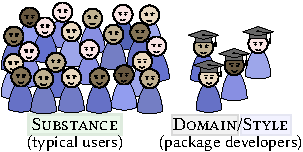
\includegraphics[scale=1.5]{assets/penrose/NoviceExpertUsers.pdf}
  \end{minipage}\hfill
\end{figure}

A secondary decision is to split specification of mathematical content and visualization across two domain-specific languages: \Substance{} and \Style{}.  A good analogy is the relationship between HTML \cite{BernersLee:1995:HML}, which specifies content, and CSS~\cite{Lie:2005:CSS}, which describes how it is rendered.  A schema called \Domain{} (analogous to XML or JSON schemas) defines the mathematical domain of interest, supporting \ref{gol:NoFixedDomains}.  In line with \ref{gol:ManyViz}, this division allows the same styles to be reused for different content, and likewise, the same content to be displayed in many different styles.  Our goal is for this division to support an ecosystem where novice users can benefit from packages written by more experienced developers (\cref{fig:NoviceExpertUsers}).  Finally, as in mathematics, the ability to adopt user-defined, domain-specific notation (\cref{sec:MathematicalDomain}) enables efficient expression of complex relationships in a way that is both concise and easy to understand~\cite{Kosar:2012:PCD}.  Encoding ideas directly in the idiom of a problem domain often results in better program comprehension than (say) a sequence of library calls in a general-purpose language~\cite{van2000domain}.  We discuss the scope and limitations of our languages in~\cref{sec:DiscussionandFutureWork}.





\subsubsection{Mathematical Domain (\Domain{})}
\label{sec:MathematicalDomain}

\begin{figure}
   \begin{minipage}[c]{.35\columnwidth}
      \vspace{5\baselineskip}\caption{One benefit of a unified framework is that different domains are easily combined.  Here, two existing packages (for meshes and set theory) were combined to illustrate that a simplicial complex \figloc{(left)} is closed with respect to taking subsets \figloc{(right)}.\label{fig:DomainInterop}}
   \end{minipage}\hfill
   \begin{minipage}[c]{.55\columnwidth}
  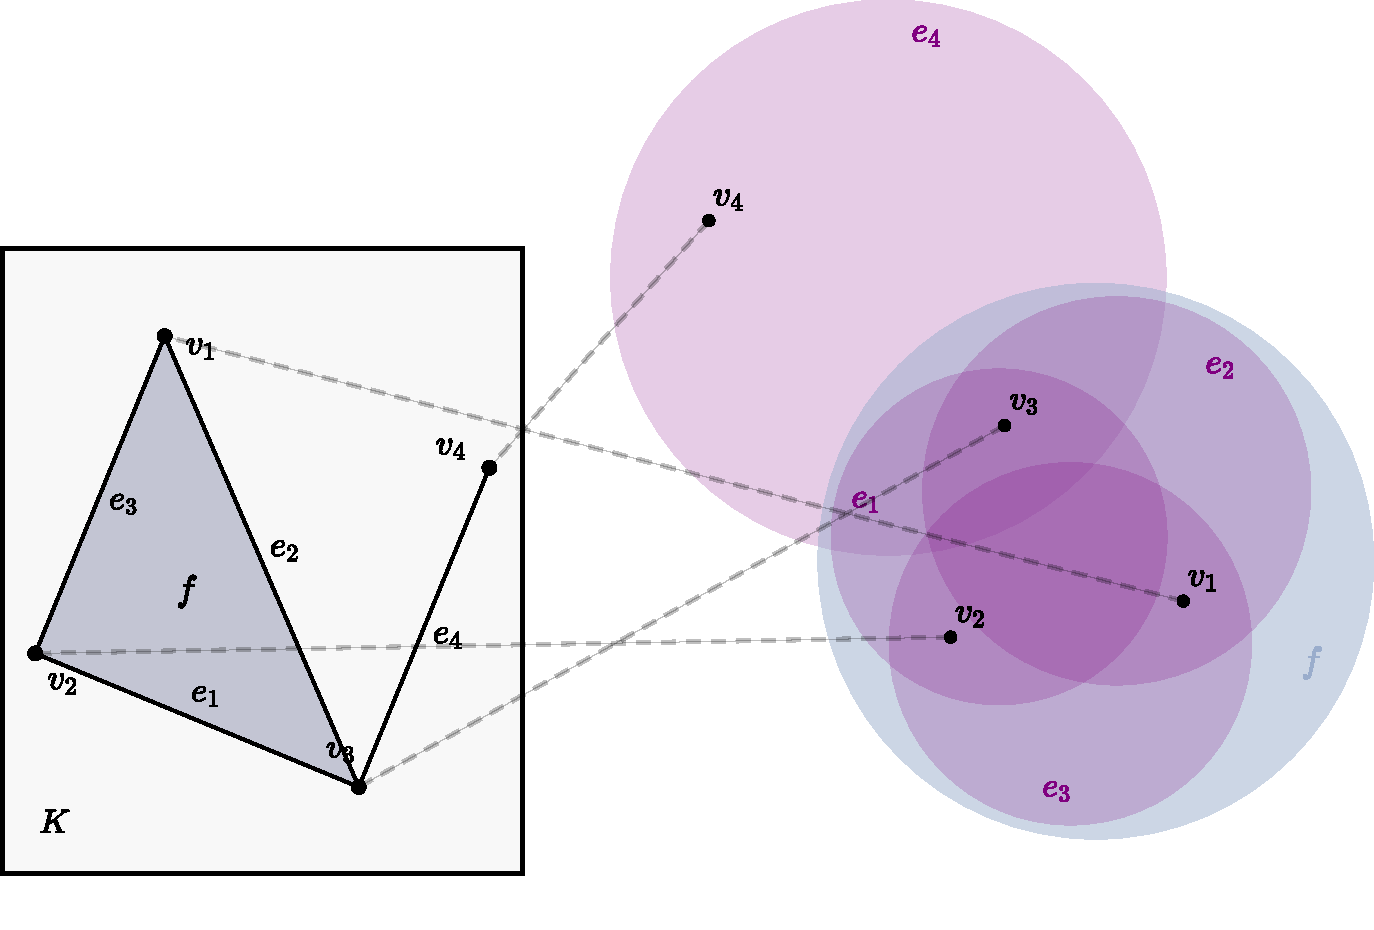
\includegraphics[width=\textwidth]{assets/penrose/domain-interop.pdf}
   \end{minipage}\vspace{-\baselineskip}
\end{figure}

One of our primary goals (\ref{gol:NoFixedDomains}) is to build a unified system for diagramming, rather than to focus on specific domains (as in, say, \emph{GraphViz}~\cite{Graphviz} or \emph{GroupExplorer}~\cite{GroupExplorer}).  A unified design enables objects from different domains to coexist in the same diagram, often by doing little more than concatenating source files (\cref{fig:DomainInterop}).  Moreover, effort put into (say) improving system performance or rendering quality is amortized across many different domains.

Users can work in any area of mathematics by writing so-called \Domain{} schemas (\cref{sec:TheDomainSchema}) that define DSLs tailored to a given domain.  This design also empowers users to adopt their own notation and conventions for modeling the domain.  Use of domain- and user-specific notation reflects common practice in mathematical writing, where the meaning of a symbol is frequently overloaded depending on context.  Importantly, a \Domain{} schema is purely abstract: it does not define an internal representation for objects, nor does it give definitions to functions or predicates.  This level of abstraction is crucial for \ref{gol:ManyViz}, since it allows multiple visual representations to later be applied to objects from the same domain.

\subsubsection{Mathematical Content (\Substance{})}
\label{sec:MathematicalContent}

% P1: What should this language look like?  Why does our design look the way it does?  Use alternatives to motivate this.
To define the content of a diagram, one must be able to specify (i) the objects in the diagram, and (ii) relationships among these objects.  In line with \ref{gol:FamiliarNotation}, \Substance{} uses concise assertions that resemble standard mathematical prose (see for example \cref{fig:MathProse}).  Formally, it can model any domain expressible in a compositional language of types, functions, and predicates, which are the basic constructs found in conventional mathematical notation~\cite{ganesalingam2013language}.  Just as definitions are typically immutable in mathematics, \Substance{} draws inspiration from strongly typed functional languages (such as \emph{ML}~\cite{Milner:1997:DSM}) where objects are stateless.  This choice also simplifies system implementation, since the compiler can assume fixed definitions.  % P2: No data, just viz!
A conscious design decision, in line with \ref{gol:ManyViz}, is to exclude all graphical data (coordinates, sizes, colors, \etc{}) from \Substance{}---since its sole purpose is to specify \emph{abstract relationships} rather than \emph{quantitative data}.  All such data is instead specified in \Style{} or determined via optimization.  This division relieves users from the burden of tedious and repetitive graphics programming, which can instead be factored out into reusable \Style{} code.

% P3: What are possible alternatives?
Existing languages would be difficult to use in place of \Substance{} since they lack the semantics needed to encode complex logical relationships and do not provide language-level extensibility.  For instance, \TeX{} \cite{Beeton:2016:CMT} and \emph{MathML} \cite{Miner:2005:IMM} markup provide only enough information to translate plain text into mathematical glyphs; computer algebra systems like \emph{Mathematica} and \emph{Maple} have limited type systems or provide only a small set of fixed predicates (\eg asserting that a number is real).  Conversely, the much richer languages used by automated theorem provers and proof assistants (such as \emph{Coq}~\cite{Bertot:2013:ITP} and \emph{Lean}~\cite{deMoura:2015:LTP}) are overkill for simply specifying diagrams. A custom language provides simple, familiar syntax and clear error messages.  We do however adopt some ideas from \emph{Coq}, such as the ability to customize syntactic sugar (\cref{sec:TheDomainSchema}).

\begin{figure}[t]
   \centering
   \hspace{-.5em}\begin{minipage}{120pt}
      \small\emph{For any vector space \(X\), let \(u, v \in X\) be orthogonal vectors of equal length, and let \(w = u+v\).  Then \(u\) and \(w\) make a \(45^\circ\) angle.}
   \end{minipage}
   \hspace{-.5em}\begin{minipage}{160pt}
  \begin{lstlisting}[language=Sub-LA,escapechar=@,numbers=none]
     VectorSpace X
     Vector u, v $\in$ X
     Orthogonal(u, v)
     EqualLength(u, v)
     Vector w $\in$ X
     w := u + v\end{lstlisting}
   \end{minipage}
   \hspace{.5em}\begin{minipage}{120pt}
      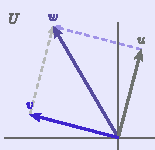
\includegraphics[width=\linewidth]{assets/penrose/MathProse.pdf}
   \end{minipage}
   \caption{Extensibility enables users to adopt conventions and notation \figloc{(center)} that reflect the way they naturally write mathematical prose \figloc{(left)}.  Here, the resulting diagram \figloc{(right)} plays the role of the concluding statement.\label{fig:MathProse}}
\end{figure}


\subsubsection{Mathematical Visualization (\Style{})}
\label{sec:MathematicalVisualization}

% The \Style{} language is used to encode a generic mapping from mathematical objects or relationships that might appear in a \Substance{} program to their visual representation.

% P1: WHAT do we specify? Constraints and objectives
The meaning of a diagram is largely conveyed by relative relationships rather than absolute coordinates.  Moreover, diagrams are often underconstrained: relationships needed to convey the intended meaning determine a \emph{family} of possible solutions, rather than a single unique diagram.  \Style{} hence adopts a constraint-based approach to graphical specification in the spirit of \emph{Sketchpad} \cite{sketchpad}: diagrams are built up from hard constraints that must be satisfied and soft penalties that are minimized (\cref{sec:ConstraintsAndObjectives}), then unspecified quantities are solved for via numerical optimization (\cref{sec:LayoutEngine}).  Though procedural definitions can still be used, the programmer need not provide absolute coordinates (as in imperative languages like \emph{PostScript} or \emph{OpenGL}).  Though an implicit specification can make output hard to predict, part of the allure of \Penrose{} is the potential to find interesting or surprising examples.  Moreover, the approach yields more concise code; for instance, \Style{} programs are much shorter than the SVG files they produce.

% P3 What are the alternatives? APIs, visual programming
An alternative design might be to use an application programming interface (API), though historically APIs have been eschewed for specification languages for good reason. Language provides far more concise expression of complex relationships---imagine styling an entire website via the DOM API's \texttt{getElementById()} and \texttt{setStyle()} methods, versus a few short lines of CSS. Visual programming languages (like \emph{LabView}~\cite{Elliott:2007:NIL} or \emph{Grasshopper}~\cite{McNeel:2010:GGM}) might suffice for basic specifications (\eg vectors should be drawn as arrows), but don't scale to more complex concepts that are easily expressed via language~\cite{Burnett:1995:SUV}.

A key design challenge is identifying objects that appear in a \Substance{} program.  Objects in a given mathematical universe are distinguished not only by their type, but also by their relationships to other objects.  A widely-used mechanism for specifying such relationships is through CSS-like \emph{selectors}. \Style{} adopts a similar mechanism that performs pattern matching on the types, functions, and predicates appearing in a \Domain{} schema (\cref{sec:Selectors}).


\subsection{Optimization-Based Synthesis}
\label{sec:OptimizationBasedSynthesis}

The second major design decision in \Penrose{} is to use constrained optimization to synthesize diagrams satisfying a given specification (\cref{sec:LayoutEngine}).  This approach is again inspired by how people often draw diagrams by hand (\eg using GUI-based tools): visual icons are placed on a canvas and iteratively adjusted until no further improvements can be made.  In difficult scenarios, a diagrammer may try several global arrangements before refining the final design, though typically no more than a few.  Automating this process makes it easy to perform layout tasks that would be tedious by hand (\cref{fig:sets-color-opt}).

\begin{figure}[h]
  \centering
  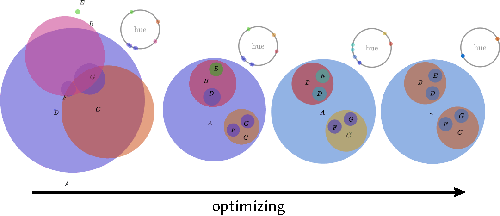
\includegraphics[scale=1.5]{assets/penrose/sets-color-opt.pdf}
  \caption{An optimization-based approach makes it possible to jointly optimize visual attributes that are difficult to coordinate by hand.  Here for instance we optimize color contrast according to the spatial proximity of adjacent disks \figloc{(left to right)}, ultimately discovering a two-color solution \figloc{(far right)}.  The system can also be used to debug the optimization process itself---in this case by drawing the hue of each disk as a dot on a color wheel.\label{fig:sets-color-opt}}
\end{figure}

There are good reasons to believe that an optimization-based approach can scale to very complex diagrams.  First, attractive diagrams need not be optimal in a \emph{global} sense---they should simply not permit obvious \emph{local} improvements, such as text that could easily be moved closer to the item it labels. In fact, disparate local minima can provide useful examples that help build intuition (\cref{fig:enumerate-subsets}).  Second, even sophisticated diagrams have surprisingly few degrees of freedom in comparison to many modern optimization problems (\eg tens or hundreds, versus thousands or millions).  Finally, strategies employed by expert diagrammers can be applied to manage complexity, such as independently optimizing small components of a diagram (akin to nonlinear Gauss-Seidel), rather than optimizing all degrees of freedom simultaneously.

In line with \ref{gol:NoFixedDomains} and \ref{gol:ManyViz}, an optimization-based approach can be applied generically and automatically for any user-defined domain and visual representation, without requiring programmers to think about the details of the layout process.  In our system, the optimization problem is defined using common-sense keywords (\cref{sec:ConstraintsAndObjectives}) in \Style\ and chaining together basic operations (\eg arithmetic).  Since the diagram specification is divorced from the details of the solver, optimization strategies can be changed and improved in future versions of the system while preserving compatibility with existing code.  The main cost of an optimization-based approach is that it puts demands on system design ``upstream'': all expressions used to define a visual style must be differentiable. As discussed in \cref{sec:Solver}, these requirements are largely satisfied via standard techniques (\eg{} by using \textit{automatic differentiation}).

\begin{figure}[t]
   \begin{minipage}[c]{.5\linewidth}
   \includegraphics{assets/penrose/enumeration.pdf}
   \end{minipage}\hfill
   \begin{minipage}[c]{.4\linewidth}
   \caption{A language-based design makes it easy to build tools on top of \Penrose{} that provide additional power. Here we use standard techniques from program synthesis (\cref{sec:LargeScaleDiagramGeneration}) to automatically enumerate how the given relationships can be realized.  Generating such examples helps to see important corner cases that might be missed when drawing diagrams by hand (where perhaps the top-left diagram most easily comes to mind).\label{fig:enumerate-subsets}}
   \end{minipage}
\end{figure}

% , and each graphical primitive must support efficient geometric queries (\eg bounding box evaluation and closest point queries). 

In general, diagram optimization is a challenging problem in its own right, which we of course do not aim to solve conclusively in this chapter.  Currently, we just use a generic constrained descent solver (\cref{sec:Solver}).  However, we have been pleased to find that this simple approach handles a wide variety of examples from different domains without requiring domain-specific strategies.


\subsection{Plugins}
\label{sec:PlugInDesign}

% TODO: Review the rewritten plugin sections

% Design decision 1: Have a plugin system for integrating external code
% Why? Further extensibility. Can't be a closed system. Lots of existing mathematical code that just needs the right interface, e.g. specialized mesh processing code.

% Decision 2. The plugin interface. A plugin receives Substance code and Style floats; outputs Substance code only (appended to file) and Style constants.
% Why? Keep it abstract, so you can use Penrose. augment set of abstract objects; provide basic information about their layout, but doesn't directly style them. Limit the power of a plugin: simplicity and modularity. 

% Decision 3. (Goes in "system" section) How to use a plugin: (Substance code JSON, Style constants as floats) -> (append Substance code as text file; output JSON for style)
% Why? JSON, floats, text files are all easy and portable, rather than calling an "API machine". Plugin can be written in any languge as long as it satisfies this inteface.

The final design decision in \Penrose\ is to provide system-level extensibility via a \textit{plugin} interface for calling external code in \Substance\ and \Style. Providing a plugin system is essential to enable users to integrate external code that is specialized to solve particular logical or graphical challenges. In fact, such interfaces for integrating external code are already provided by many systems (\eg \TeX, \emph{Adobe Illustrator}, and TikZ's plugin system for graph layout algorithms~\cite{Graphviz}). The interface for \Penrose\ plugins is designed to define a clear and simple boundary between the \Penrose\ system and the plugin while enabling each component to focus on its strengths. A plugin can analyze and augment the set of abstract objects defined in \Substance\, as well as analyze and augment the numerical information in \Style. This simple interface allows plugins to be written in any language (or repurposed from other systems) and operate independently from the implementation details of \Penrose. However, a plugin cannot change an existing \Substance\ or \Style\ program or directly generate static graphical content, since such plugins would abandon the benefits that \Penrose{} provides, such as the ability to re-style content and avoid use of absolute coordinates. \cref{fig:Retargeting} illustrates how a simple plugin can make use of \Substance\ and \Style\ information to create ``responsive'' diagrams.

% Since the \Penrose\ system focuses on diagram specification and synthesis, it does not natively perform sophisticated logical reasoning for \Substance\ programs. Additionally, we want to provide a way for users to avoid reinventing the wheel when it comes to graphical layout in \Style.


\section{Language Framework}
\label{sec:LanguageFramework}

The \Penrose{} language framework comprises three languages that play different roles:

\begin{itemize}
   \item A \inlineDSL{\Domain{} schema} declares the objects, relationships, and notation available in a mathematical domain.
   \item A \inlineSUB{\Substance{} program} makes specific mathematical assertions within some domain.
   \item A \inlineSTY{\Style{} program} defines a generic mapping from mathematical statements in some domain to a visual representation.
\end{itemize}

A \emph{package} consisting of a \(\Domain{}\), and one or more compatible \(\Style{}\) programs, can be used to illustrate \Substance{} programs from a given domain (\cref{fig:HighLevelPipeline}).  Though some starter packages are provided for the examples discussed in~\cref{sec:ExamplesandEvaluation}, the real power of \Style{} and \Domain{} is that they enable \Penrose\ to be easily extended.  In this section we illustrate these languages via the running example of a linear algebra package (Figures~\ref{fig:domain_linalg} through \ref{fig:style_linalg}).  Formal grammars for the three languages are given in supplemental material.



\subsection{The \Domain{} Schema}
\label{sec:TheDomainSchema}

A \Domain{} \emph{schema} describes a domain of mathematics by defining the objects and notation that can be used by associated \Substance{} and \Style{} programs.  A partial example for linear algebra is shown in \cref{fig:domain_linalg} (the full schema is provided in supplemental material).  The \inlineDSL{\keyword{type}} lines define the available object types, \inlineDSL{\keyword{function}} lines define the domain and codomain for the set of available functions (where \texttt{*} denotes a Cartesian product), and \inlineDSL{\keyword{predicate}} lines define the possible relationships among objects, including unary predicates.  Importantly, a \Domain{} schema is purely abstract: it does not define a specific representation for objects, nor does it define bodies for functions or predicates. For instance, we do not say here that a vector is encoded by a list of coordinates, nor do we write an addition operation on such coordinates.  A concrete visual interpretation of these definitions is given by a \Style{} program (\cref{sec:TheStyleLanguage}).  Types can be given fields via \emph{constructors}. For instance, the line
\[
   \text{\small\texttt{\textbf{constructor} MakeInterval: Real min * Real max -> Interval}}
\]
assigns fields \texttt{min} and \texttt{max} to an \texttt{Interval}, which can be accessed from a \Substance{} or \Style{} program (\eg to assert a relationship between endpoints).  Subtyping via the syntax \texttt{Subtype <: Type} facilitates generic programming.  Finally, \inlineDSL{\keyword{notation}} lines define optional syntactic sugar that can simplify code (\eg in \cref{fig:substance_linalg}).

\begin{figure}
\begin{mdframed}[style=DSLCode]
\begin{lstlisting}[language=Elem,escapechar=@]
type Scalar, VectorSpace, Vector      -- LinearAlgebra.dsl @\label{lin:linalg_types}@
function add: Vector * Vector -> Vector @\label{lin:linalg_functions_begin}@
function norm: Vector -> Scalar
function scale: Scalar * Vector -> Vector
... @\label{lin:linalg_functions_end}@
predicate In: Vector * VectorSpace @\label{lin:linalg_predicates_begin}@
predicate Unit: Vector
predicate Orthogonal: Vector * Vector
... @\label{lin:linalg_predicates_end}@
notation "v1 + v2" $\sim$ "add(v1,v2)"
notation "|y1|" $\sim$ "norm(y1)"
notation "s * v1" $\sim$ "scale(s,v1)"
notation "Vector v $\in$ V" $\sim$ "Vector a; In(a,U)"
notation "v1 $\perp$ v2" $\sim$ "Orthogonal(v1,v2)"
...
\end{lstlisting}
\end{mdframed}
   \caption{A \Domain{} schema specifies the building blocks available in a given mathematical domain, as well as any associated syntactic sugar.  This schema (abbreviated) enumerates some basic constructs from linear algebra.\label{fig:domain_linalg}}
\end{figure}


\subsection{The \Substance{} Language}
\label{sec:TheSubstanceLanguage}

Each statement in the \Substance\ language either (i) declares an object, (ii) specifies properties of an object, or (iii) specifies relationships among objects within some \Domain{} schema.  As in mathematics, not all attributes need be fully specified. For instance, one can talk about a point without giving it explicit coordinates. Together, these statements describe a \emph{context} that encloses all the mathematical objects and relationships that have been defined.

\begin{figure}
\begin{minipage}[!t]{140pt}
\begin{mdframed}[style=SUBCode]
\begin{lstlisting}[language=Sub-LA,escapechar=@,numbers=none]
VectorSpace X
Vector x1, x2
In(x1, X)
In(x2, X)
Unit(x1)
Orthogonal(x1, x2)
label x1 @$\$$@x_1@$\$$@
label x2 @$\$$@x_2@$\$$@
\end{lstlisting}
\end{mdframed}
\centering (unsugared)
\end{minipage}
\hfill
\begin{minipage}[!t]{150pt}\vspace{-2\baselineskip}
\begin{mdframed}[style=SUBCode]
\begin{lstlisting}[language=Sub-LA,escapechar=@,numbers=none]
VectorSpace X
Vector x1, x2 $\in$ X
Unit(x1)
x1 $\perp$ x2
label x1 @$\$$@x_1@$\$$@
label x2 @$\$$@x_2@$\$$@
\end{lstlisting}
\end{mdframed}
\centering (sugared)
\end{minipage}
\hfill
\begin{minipage}[!t]{150pt}
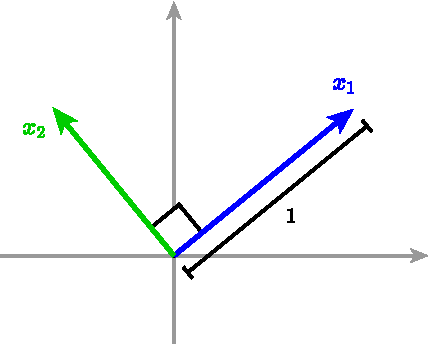
\includegraphics[width=1\columnwidth]{assets/penrose/substance-linalg.pdf}
\end{minipage}
   \caption{When used with the \Style{} defined in \cref{fig:style_linalg}, this \Substance{} code (with or without syntactic sugar) produces the diagram shown at right.\label{fig:substance_linalg}}
\end{figure}

\cref{fig:substance_linalg} shows an example in which \Substance{} code specifies properties and relationships for a pair of vectors.  Importantly, these statements do not induce any kind of numerical evaluation.  For instance, no coordinates are assigned to \texttt{x1} in order to make it unit---in fact, the vector space \texttt{X} does not even have an explicit dimension.  Instead, statements specify persistent and purely symbolic relationships that provide cues for visualization;  specific coordinates and attributes are later determined by the layout engine (\cref{sec:LayoutEngine}). The final lines specify label strings to be used by the \Style{} program, here in \TeX{} notation.  \cref{fig:substance_linalg}, \figloc{center} shows a ``sugared'' version of this program using notation defined in the \Domain{} schema (\cref{fig:domain_linalg}).  Users can write programs either way, depending on the capabilities of their editor (\eg support for Unicode input).


\subsection{The \Style\ language}
\label{sec:TheStyleLanguage}

% TODO Add brief discussion of layering

% TODO Add brief discussion of transforms, "then" keyword

\setlength{\columnsep}{1em}
\setlength{\intextsep}{1em}
\begin{wrapfigure}{l}{200pt}
   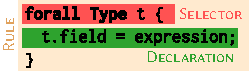
\includegraphics[width=\linewidth]{assets/penrose/StyleNomenclature.pdf}
\end{wrapfigure}
\Style{} specifies how expressions in a \Substance{} program are translated into graphical objects and relationships.  It is a declarative specification language that shares many features with CSS.  The core principle is to sketch out basic \emph{rules} (\eg visual icons for basic types) and then refine these rules via \emph{cascading} (\cref{sec:Cascading}).  Each rule uses a \emph{selector} to pattern match on objects and relationships appearing in \Substance{} code (\cref{sec:Selectors}).  A sequence of \emph{declarations} then specifies a corresponding visualization, \eg by emitting graphical primitives or enforcing constraints.  Each declaration either assigns a \emph{value} to a \emph{field} (\cref{sec:ValuesAndExpressions,sec:Fields}) or specifies a \emph{constraint} or \emph{objective} (\cref{sec:ConstraintsAndObjectives}).  An example is shown in \cref{fig:style_linalg}, which defines part of the style used for the \Substance{} program in \cref{fig:substance_linalg} (a full \Style\ is given in the supplemental material).  We will use this example to highlight the basic features of the language.  

\begin{figure}[p]
\begin{mdframed}[style=STYCode]
\begin{lstlisting}[language=Sty-LA,escapechar=@]
forall VectorSpace U {                    -- LinearAlgebra.sty@\label{lin:VectorSpaceRule}@
   U.originX = ? -- to be determined via optimization
   U.originY = ? -- to be determined via optimization
   U.origin = (U.originX, U.originY)
   U.xAxis = Arrow { -- draw an arrow along the x-axis
          startX : U.originX - 1 @\label{lin:VSArrowGeometryBegin}@
          startY : U.originY
          endX   : U.originX + 1
          endY   : U.originY @\label{lin:VSArrowGeometryEnd}@
      thickness  : 1.5 @\label{lin:VectorSpaceConstantsBegin}@
          style  : "solid"
          color  : Colors.lightGray @\label{lin:VectorSpaceConstantsEnd}@
   } -- (similar declarations omitted for the y-axis)
}
forall Vector u, VectorSpace U where In(u, U) { @\label{lin:VectorElementRule}@            
   u.arrow = Arrow { @\label{lin:VectorIsALittleArrow}@
      startX : U.originX @\label{lin:VectorArrowStart}@
      startY : U.originY
        endX : ? @\label{lin:PendingArrowEnd}@
        endY : ?
       color : Colors.mediumBlue
   } @\label{lin:VectorIsALittleArrowEnd}@
   u.text = Text {
      string : u.label -- label from Substance code
       color : u.arrow.color @\label{lin:VectorLabelColor}@ -- use arrow's color
   }
   u.start = (u.arrow.startX, u.arrow.startY)
   u.end = (u.arrow.endX, u.arrow.endY)
   u.vector = minus(u.arrow.end, u.arrow.start) @\label{lin:VectorVector}@
   encourage near(u.text, u.end) @\label{lin:LabelObjective}@
   ensure contained(u.end, U.shape)
}
forall Vector u, Vector v @\label{lin:OrthogonalSelector}@
where Orthogonal(u, v) { @\label{lin:OrthogonalRule}@
   local.perpMark = Curve { @\label{lin:OrthogonalShape}@
        pathData : orientedSquare(u.shape, v.shape, U.origin, const.perpLen)
        strokeWidth : 2.0
        color : Colors.black
        fill : Colors.white
   } @\label{lin:OrthogonalShapeEnd}@
   ensure equals(dot(u.vector, v.vector), 0.0) @\label{lin:OrthogonalConstraint}@
}
... -- (similar rule omitted for Unit)
Vector `x2` @\label{lin:VectorBacktick}@ { override `x2`.shape.color = Colors.green; @\label{lin:OverrideVectorColor}@ }
\end{lstlisting}
\end{mdframed}
   \vspace{-.5\baselineskip}\caption{The \Style{} program defining the visual style used in \cref{fig:substance_linalg}, \figloc{right}. Note that this \Style{} program can be reused for many different \Substance{} programs in the same domain.\label{fig:style_linalg}}
   
\end{figure}

\subsubsection{Selectors}
\label{sec:Selectors}

A selector uses pattern matching to specify which objects will be styled by a rule.  Unlike regular expressions, selectors do not match literal strings of \Substance{} code, but rather objects and relationships in the context defined by this code.  A simple example is a selector that matches every instance of a type, indicated by the \inlineSTY{\keyword{forall}} keyword.  For instance, \cref{lin:VectorSpaceRule} matches all vector spaces.  In subsequent declarations, \inlineSTY{\texttt{U}} refers to the vector space \inlineSUB{\texttt{X}} from the \Substance\ program.  The \inlineSTY{\keyword{where}} keyword restricts matches to objects that satisfy one or more relationships; \eg \cref{lin:OrthogonalRule} matches all pairs of orthogonal vectors.  One can also match by name using backticks; \eg \cref{lin:VectorBacktick} matches only the vector \inlineSUB{\texttt{x2}}.  Selectors could be enriched in the future to allow other statements from first-order logic (such as \(\exists\), disjunctions, and conjunctions).

\subsubsection{Cascading}
\label{sec:Cascading}

A cascading mechanism allows rules to be refined for more specialized objects or relationships.  For example, the selector in \cref{lin:VectorBacktick} matches a specific vector, refining an earlier rule that applies to all vectors.  Rule precedence is determined by order in the \Style{} file, and later rules can refer to any previously defined \emph{field} (\cref{sec:Fields}).  The \inlineSTY{\keyword{override}} keyword (\cref{lin:OverrideVectorColor}) hints that a rule will modify an existing field, otherwise the compiler issues a warning.


\subsubsection{Fields}
\label{sec:Fields}

The visual representation of an object is specified by creating \emph{fields} that are assigned \emph{values} (\cref{sec:ValuesAndExpressions}).  For instance, in Lines \ref{lin:VectorIsALittleArrow}--\ref{lin:VectorIsALittleArrowEnd} a field called \inlineSTY{\texttt{u.arrow}} is created and assigned an expression describing an arrow.  Fields are created on assignment and can have any name not conflicting with a reserved word.  Fields not naturally associated with a single object can also be assigned locally to a rule. For instance, \cref{lin:OrthogonalShape} is used to draw a right angle mark between any pair of orthogonal vectors.  Every object automatically has fields \inlineSTY{\texttt{name}} and \inlineSTY{\texttt{label}} storing its \Substance{} name and label string (\resp), as well as any field created via a constructor (\cref{sec:TheDomainSchema}).


\subsubsection{Properties}
\label{sec:Properties}

\Style{} provides built-in graphical primitives (circle, arrow, \etc{}) with a fixed set of \emph{properties}. Like fields, properties can be assigned values (as in Lines~\ref{lin:OrthogonalShape}--\ref{lin:OrthogonalShapeEnd}). If a value is not assigned, it will be assigned a default value, possibly a \emph{pending value} (\cref{sec:ValuesAndExpressions}).  For example, an arrow might be black by default, whereas the width of a box might be optimized (akin to \emph{flexible space} in \TeX).

% Note that the set of graphical primitives is easily extensible (or indeed, the entire rendering frontend), though we do not currently expose such extensibility at the language level.

\subsubsection{Values and Expressions}
\label{sec:ValuesAndExpressions}

Atomic \emph{values} can be combined to form \emph{expressions}.  For instance, Lines \ref{lin:VectorSpaceConstantsBegin}--\ref{lin:VectorSpaceConstantsEnd} assign values, whereas Lines \ref{lin:VSArrowGeometryBegin}--\ref{lin:VSArrowGeometryEnd} assign composite expressions involving inline computation.  \cref{lin:VectorLabelColor} specifies value via a \emph{path}, \ie, a sequence of expressions separated by \inlineSTY{\texttt{.}} characters; such assignments are made by reference.  Expressions can also access values from plugins (\cref{sec:PlugIns}).  A very important construct is \emph{pending values}, denoted by a \inlineSTY{\texttt{?}} as in \cref{lin:PendingArrowEnd}.  This line specifies that the location of the arrow endpoint is not fixed and will be automatically determined by the solver (\cref{sec:LayoutEngine}).

\subsubsection{Constraints and Objectives}
\label{sec:ConstraintsAndObjectives}

Constraints and objectives describe how pending values should behave.  In particular, the \inlineSTY{\keyword{ensure}} keyword defines a hard constraint that the diagram must satisfy. For instance, \cref{lin:OrthogonalConstraint} specifies that two orthogonal vectors must be drawn at right angles.  The \inlineSTY{\keyword{encourage}} keyword specifies a relationship that should be satisfied as much as possible. For instance, \cref{lin:LabelObjective} asks that the label for a vector be placed close to its endpoint. These expressions are translated into constraints and energy functions that make up a numerical optimization problem (\cref{sec:Solver}).


\section{Layout engine}
\label{sec:LayoutEngine}

\begin{figure}[t]
  \centering
  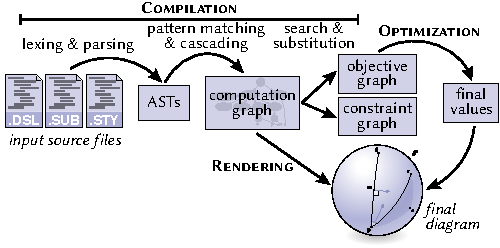
\includegraphics[scale=1.5]{assets/penrose/CompilationPipeline.pdf}
	\caption{Pipeline view of the layout engine.  Rather than a single static image, compilation yields an optimization problem that can be solved and re-solved to produce many diagrams, or (in principle) used in an interactive tool.\label{fig:CompilationPipeline}}
\end{figure}


% (SOURCE [.dsl,.sub,.sty]) ---- "compilation" ----> OPTIMIZATION PROBLEM ---- optimization ----> DIAGRAM
% TODO Turn the ASCII art above into a real diagram that explains (at an appropriate level of granularity) the steps of the Engine

% ENGINE
%  (static compilation)
%    1 check correctness of .dsl
%    2 check correctness of .sub using .dsl
%    3 check correctness of .sty using .dsl
%  (dynamic compilation)
%    4 build dictionary from .sub to .sty
%    5 apply dictionary to transform .sub program into "pre-diagram" + initial guess for unknown state
%       5a Fill in some unknown attributes deterministically (e.g., using defaults or random samples)
%    6 build optimization problem that solves for unknowns in pre-diagram
%  (optimization)
%    7 solve optimization problem
%    8 render the diagram

The layout engine translates \Penrose{} code into images (\cref{fig:CompilationPipeline}).  There are two main stages: a compiler (\cref{sec:Compiler}) translates code into an optimization problem that describes possible diagrams, then a solver (\cref{sec:Solver}) produces solutions to this problem. These values are used to render the final diagram (\cref{sec:Rendering}). For simplicity, the goal is to automatically produce one static diagram, but the same pipeline could be extended to support capabilities like interaction.

% These stages of diagram generation are exposed in a standard Application Programming Interface (API).

\subsection{Compiler}
\label{sec:Compiler}

The input to the compiler is a triple of files: a \Domain{} schema with \Substance{} and \Style{} programs.  The output is a constrained optimization problem, expressed as a computational graph.

\subsubsection{Parsing and Type Checking}
\label{sec:ParsingandTypeChecking}

We parse each of the input files into abstract syntax trees (ASTs), applying static typechecking to ensure that types are well-formed and variables are well-typed.  We first typecheck the \Domain{} program since it defines the valid types for the \Substance{} and \Style{} programs, then use these types to check the \Substance{} program and the selectors in the \Style{} code.
% Our implementation uses a \emph{parser combinator} approach~\cite{Swierstra:2001:CPF}.

\subsubsection{Computational Graph}
\label{sec:ComputationalGraph}

The ASTs are combined to define a \emph{computational graph} that encodes operations that define the final diagram (\cref{fig:build_computation_graph}).  To build this graph, we apply a standard pattern matching and cascading procedure: iterate over rules in the \Style{} program, find tuples of \Substance{} variables that match the selector pattern, then modify the graph according to the declarations within the matched rule.  For example, when the first selector \inlineSTY{\texttt{\textbf{VectorSpace} U}} from \cref{fig:style_linalg} matches the variable \inlineSUB{\texttt{X}} from \cref{fig:substance_linalg}, we add nodes to the graph that encode the axes of this vector space.  In general, declarations could also remove nodes from the graph or connect previously added nodes.  Once this transformation is complete, we have replaced all abstract mathematical descriptions with concrete graphical representatives.  All that remains is to determine pending values (\ie{}, those marked by a \inlineSTY{\texttt{?}}) and those values that depend on them, which will be done by the solver.

% Compiler output example: \texttt{https://gist.github.com/hypotext/7895b8e7e1abbe62f5abe84efbc036d6} 

\subsubsection{Optimization Graphs}
\label{sec:OptimizationGraphs}

\begin{figure}
   \begin{minipage}[c]{.4\linewidth}
      \vspace{-\baselineskip}\caption{Applying the mapping defined by \Style{} code to a \Substance{} program yields a graph that describes how to draw the diagram---here, for part of \cref{fig:substance_linalg}.  Some values are known (in blue), whereas others (in orange) depend on unknowns that must be determined via optimization.\label{fig:build_computation_graph}}
   \end{minipage}\hfill
   \begin{minipage}[c]{.5\linewidth}
   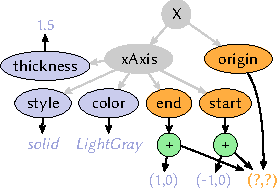
\includegraphics[scale=1.5]{assets/penrose/build_computation_graph.pdf}
   \end{minipage}
\end{figure}

\begin{figure}[t]
\centering
   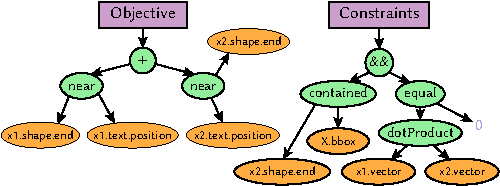
\includegraphics[scale=1.5]{assets/penrose/optimization_computation_graph.pdf}
   \caption{The computation graph is further expanded to produce graphs representing the objective and constraint space for our optimization problem. From there, we can easily use automatic differentiation to obtain derivatives.  This figure depicts part of the optimization graph for \cref{fig:substance_linalg}.\label{fig:optimization_computation_graph}}
 \end{figure}
 % \setlength{\belowcaptionskip}{-30pt}

 
 To encode the optimization problem, we collect terms from the computational graph into an objective and constraint graph (\cref{fig:optimization_computation_graph}). Each \inlineSTY{\keyword{ensure}} and \inlineSTY{\keyword{encourage}} statement is then replaced by the corresponding mathematical expression.  For instance, \inlineSTY{\texttt{\textbf{ensure} equal(x,y)}} is translated into the constraint \(x-y=0\), which the solver seeks to enforce exactly, whereas \inlineSTY{\texttt{\textbf{encourage} equal(x,y)}} becomes the objective \((x-y)^2\), which the solver seeks to minimize as much as possible.  The overall constraint set is the intersection of all constraints, and the overall objective is a sum of objective terms. Currently \Penrose{} provides a fixed set of constraints and objectives, though it would be straightforward to extend \Style{} to allow user-defined inline expressions.

% TODO Show computational graph for linear algebra example

\subsection{Solver}
\label{sec:Solver}

The optimization graphs produced by the compiler describe an optimization problem in standard form, \ie, minimization of an objective function subject to equality and inequality constraints~\cite[Section 4.1]{Boyd:2004:CO}.  Such problems may be solved with many standard methods. We currently use an \emph{exterior point method}~\cite{Yamashita:2010:PDE} that starts with an infeasible point and pushes it toward a feasible configuration via progressively stiffer penalty functions---mirroring a process often used by hand (\cref{sec:OptimizationBasedSynthesis}).  Moreover, the exterior point mehod is an appropriate choice since (i) a feasible starting point is typically not known (\cref{fig:OptimizationProgress}), and (ii) by converting constraints into progressively stiffer penalty functions, we can use descent algorithms that do not directly support constrained optimization.  In particular, we use L-BFGS with a line search strategy suitable for nonsmooth objectives~\cite{Lewis:2009:NOB}.  Given the rich structure of our optimization graphs, which can be linked back to program semantics, there are plenty of opportunities to improve this generic strategy, such as decomposing the problem into smaller pieces that can be independently optimized, or employing an SMT solver to find a feasible initial state.

\begin{figure}[t]
   \centering
   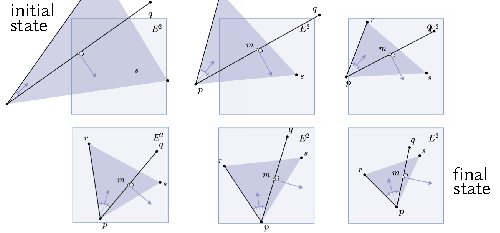
\includegraphics[scale=1.5]{assets/penrose/OptimizationProgress.pdf}
   \caption{Our solver can lay out diagrams even if we do not initially know how to satisfy all the constraints. Here we show several steps of optimization.\label{fig:OptimizationProgress}}
\end{figure}

\subsubsection{Initialization}

Just as a human diagrammer might consider several initial arrangements, we randomly sample several configurations and optimize only the most promising ones, \ie, the ones with the least overall energy in the exterior point problem.  Initial values are sampled uniformly at random from a range related to their types; for example, RGB color values are sampled from \([0,1]\).

\subsubsection{Failures and warnings}

Since our language framework is quite general, a programmer might define difficult or impossible optimization problems.  Hence, we can't guarantee that \Penrose{} produces a valid diagram.  However, the system can provide feedback by simply printing an error message if any of the constraint values are nonzero.  The resulting invalid diagram might even provide useful visual intuition for why the \Style\ program failed (\cref{fig:sets-inconsistent}).

\subsection{Plugins}
\label{sec:PlugIns}

A plugin is a piece of external code, written in any language, that is given information from a specific pair of \Substance\ and \Style\ files and can produce more \Substance\ and \Style\ information in specific files for \Penrose\ to use. A plugin is run when making diagrams with a particular \Style. A \Style\ may declare the plugins to be called at the top of the file with the syntax \mbox{\inlineSTY{\texttt{plugin "myPlugin" (args)}},} which states that the plugin \inlineSTY{\texttt{myPlugin}} should be run with the given argument list. When a diagram is generated, the plugin is given the \Substance{} program as a JSON file, as well as the parameters given in \Style\ as command-line arguments. The plugin can output new \Substance\ code as a text file and/or a set of values for the fields of any \Substance\ variable, encoded as a JSON file. The \Substance\ code generated by a plugin is appended to the existing \Substance\ program, and the values generated by the plugin can be accessed in \Style{} via the syntax \inlineSTY{\texttt{myPlugin[variable][field]}}. Note that a plugin is run exactly once, prior to execution of all \Penrose{} code. Therefore, the values generated by a plugin are not optimized by the layout engine, so plugin code does not have to be differentiable. For examples of plugin use, see \cref{sec:Functions} and \cref{sec:Meshes}.

% , including those \Substance\ variables generated by the plugin itself

\subsection{Rendering}
\label{sec:Rendering}

In this chapter we focused on generating 2D vector graphics, but in principle nothing about our system design limits us to this particular target.  For instance, the constraint-based approach is just as suitable for, say, generating arrangements of 3D objects that can be rendered via photorealistic ray tracing~\cite{Pharr:2016:PBR}, or even constrained interactive diagrams that could be used in virtual reality.  In our current implementation, graphical primitives are translated to SVG-native primitives via \emph{React.js}~\cite{Facebook:2020:RJS} and labels are postprocessed from raw \TeX\ to SVG paths using MathJax~\cite{Cervone:2012:MJ}.  Since \Penrose{} code is typically quite concise, we embed it as metadata into the SVG, easing reproducibility.  We also embed \Substance\ names as tooltips to improve accessibility.

\begin{figure}[t]
   \includegraphics[width=\columnwidth]{assets/penrose/PenroseIDE.jpg}
   \caption{Our system supports integration with web-based applications. Here a \Penrose\ IDE provides automatic syntax highlighting and autocomplete for any user-defined domain.\label{fig:PenroseIDE}}
\end{figure}

\subsection{Development Environment}
\label{sec:DevelopmentEnvironment}

To facilitate development, we built a web-based IDE (\cref{fig:PenroseIDE}) that highlights the potential for high-level diagramming tools built on \Penrose{}. For instance, since the \Domain{} grammar has a standard structure, the IDE can provide features like autocomplete and syntax highlighting for any domain. We are optimistic that the design choices made in \cref{sec:SystemDesign} will support the use of \Penrose{} as a platform for building diagramming tools beyond the use cases in this chapter.

 % and the ability to interactively manipulate elements of a generated diagram.
% Here, for instance, diagram elements can be dragged around the canvas and re-optimized to preserve the constraints (and hence meaning) of the given programs.  

\subsection{Implementation}
\label{sec:Implementation}

The \Penrose\ system is written in Haskell and the rendering frontend is written in Typescript. We wrote our own solver using the Haskell library \textit{ad}~\cite{autodiff:kmett} to perform automatic differentiation. We provide one output target and renderer (SVG), together with a fixed set of graphical primitives that are loosely based on SVG (\eg circles and paths), plus features that SVG users commonly add by hand, like arrowheads. We also provide a fixed set of objectives and constraints for specifying spatial layout, such as shape containment and adjacency relationships, and other functions for performing spatial queries, such as computing bounding boxes and pairwise distances. Sustained use by a community of users might point the way to a standard library. The system has been open-sourced here: \texttt{github.com/penrose/penrose}


\section{Examples and Evaluation}
\label{sec:ExamplesandEvaluation}

% GENERAL POINTS ABOUT EXAMPLES

% What are the *claims* that our examples support?
% First: there are several far-reaching claims on the first page… this approach has several broad-reaching benefits.
% Do our examples support those claims?
% Claim 1 (novices and notation). If we look at our examples, do they support this claim?
%     How do you convince someone this is familiar notation? Show snippets from some other textbook
%     Mention those four bullet points whenever we can
%     What you want to do is cut to the chase. Make the topic sentence about the system, and everything else a “for example.”
%     Make it clear that this is just an *example* and that it’s being used to illustrate a particular principle. Indicate that with phrases like "For example," "for instance," "to illustrate this principle," "just one example is"… They’re not really the example you’re talking about, just the supporting evidence. (?)

% Other example sections in systems papers:
% Section 5.2 https://arxiv.org/pdf/1910.02993.pdf
% Section 5.2 http://graphics.stanford.edu/papers/scanner/poms18_scanner.pdf

% \todo{Revise this introduction to discuss the broad claims}

Our main goal for \Penrose\ was to create a system that can automatically generate diagrams from many different domains using familiar syntax. Here we examine our design by exploring examples from a variety of common domains in mathematics and computer graphics; we also do some basic performance analysis (\cref{sec:PerformanceEvaluation}). 

% All examples in the paper were generated automatically and were not manipulated by hand. However, due to small errors when converting our SVG output to the PDF format required by \texttt{pdflatex}, minor manual editing was required (\eg{} fixing broken transparency).

% Though this process, we see that \Penrose{} programs allow us codify best practices of expert diagrammers in a way that be easily reused by non-expert users.
% ^ I'm not sure if we can support this claim...

% TODO Say something like: Being able to make lots of diagrams easily makes it that much easier to make "microdiagrams" that clearly illustrate one small idea, rather than feeling like diagrams have to be saved for only the most critical concepts, or packed full of lots of different ideas.

% TODO Discuss package used to draw our computational graphs; draw a comparison to GraphViz, pointing out that our general solution easily provides much of the core functionality of their entire specialized solution (at least from a language point of view).

\subsection{Sets}
\label{sec:Sets}

\setlength{\columnsep}{1em}
\setlength{\intextsep}{0em}
\begin{wrapfigure}{l}{140pt}
   \includegraphics[width=\linewidth]{assets/penrose/ExponentialGrowth.pdf}
\end{wrapfigure}\vspace{-\baselineskip}

A simple example that illustrates many principles of our system design is the domain of basic set theory---\cref{fig:set-styles} shows a complete listing for one of three possible styles.  Notice here the complete absence of explicit coordinates in both the \Substance{} and \Style{} code.  The other two \Style{} programs (not shown) either improve the visual styling, or shift to a different representation where subset inclusion is indicated by a tree-like drawing rather that overlapping disks.  Different representations are especially helpful for different types of examples---for instance, disks must shrink exponentially for deeply nested subsets, whereas a tree diagram remains easy to read (see inset, \textit{left}). One limitation highlighted by this example is that the constraints and objectives appearing in \Style{} are not yet extensible within the language itself---for instance, the statement \inlineSTY{\keyword{ensure} \texttt{contains(y.shape,x.shape)}} translates to a fixed function on the centers and radii of the two disks.

This example also demonstrates the benefit of a more explicit type system, rather than, say, interpreting raw mathematical strings as in \TeX.  In particular, \cref{fig:enumerate-subsets} shows how a \Domain{} schema can be used with program synthesis techniques (\cref{sec:LargeScaleDiagramGeneration}) to automatically enumerate different \emph{logical} instantiations of the given \Substance{} code.  To make this example, there was no need to model sets as an explicit datatype (\eg\ a list of points) nor to assign semantics to these datatypes (such as the impossibility of two sets being both intersecting and nonintersecting). Instead, the program synthesizer can reason purely about the abstract types specified in the \Domain\ schema, letting the constraints defined in the \Style{} define the visual semantics. Thus, the program synthesizer can check if the generated code is valid by simply testing if the constraints defined in \Style{} all evaluate to zero for the optimized diagram.  This example captures an important aspect of our system design: the mapping defined by \Style{} programs not only provides a superficial visual interpretation, but also assigns deeper mathematical meaning.

\begin{figure}[ph]
\begin{minipage}[t]{\columnwidth}
\begin{mdframed}[style=DSLCode]
\begin{lstlisting}[language=Elem,escapechar=@,numbers=none]
type Set                                   -- Sets.dsl
predicate Intersecting : Set s1 * Set s2
predicate IsSubset : Set s1 * Set s2
predicate Not : Prop p
notation "A $\subset$ B" ~ "IsSubset(A, B)"
notation "A $\cap$ B = $\varnothing$" ~ "Not(Intersecting(A, B))"
\end{lstlisting}
\end{mdframed}
\end{minipage}
\begin{mdframed}[style=SUBCode]
\begin{minipage}[t]{0.5\columnwidth}
\begin{lstlisting}[language=Sub-SET,escapechar=@,numbers=none]
Set A, B, C, D, E, F, G
B $\subset$ A
C $\subset$ A
D $\subset$ B
E $\subset$ B
\end{lstlisting}
\end{minipage}
\ContinueLineNumber
\begin{minipage}[t]{.45\columnwidth}
\begin{lstlisting}[language=Sub-mesh,escapechar=@,numbers=none]
F $\subset$ C       -- Sets.sub
G $\subset$ C
E $\cap$ D = $\varnothing$
F $\cap$ G = $\varnothing$
B $\cap$ C = $\varnothing$
\end{lstlisting}\end{minipage}\end{mdframed}
\vspace{-.9\baselineskip}
\begin{minipage}[t]{\columnwidth}
\begin{mdframed}[style=STYCode]
\begin{lstlisting}[language=Sty-ST,escapechar=@,numbers=none]
forall Set x {                       -- Sets-Disks.sty
    x.shape = Circle { strokeWidth : 0.0 }
    x.text = Text { string : x.label }
    ensure contains(x.shape, x.text)
    encourage sameCenter(x.text, x.shape)
    layer x.shape below x.text
}
forall Set x; Set y
where IsSubset(x, y) {
    ensure contains(y.shape, x.shape)
    ensure smallerThan(x.shape, y.shape)
    ensure outsideOf(y.text, x.shape)
    layer x.shape above y.shape
    layer y.text below x.shape
}
forall Set x; Set y
where NotIntersecting(x, y) {
    ensure disjoint(x.shape, y.shape)
}\end{lstlisting}\end{mdframed}\end{minipage}
\begin{minipage}[t]{\columnwidth}
\includegraphics[width=\columnwidth]{assets/penrose/set-styles.pdf}
\end{minipage}
   \caption{Here, some \Substance{} code is used to specify set relationships. Different \Style{} programs not only tweak the visual style (\eg flat vs. shaded disks), but allow one to use a completely different visual representation (\eg a tree showing set inclusions).  \texttt{Sets.sty} above describes the flat disk style.\label{fig:set-styles}}
\end{figure}


\subsection{Functions}
\label{sec:Functions}

\begin{figure}
   \centering
   \begin{minipage}[t]{0.33\columnwidth}
      \begin{mdframed}[style=SUBCode]
      \begin{lstlisting}[language=Sub-ST,escapechar=@,numbers=none]
-- Injection.sub
Set A, B
f: A -> B
Injection(f)
Not(Surjection(f))\end{lstlisting}
      \end{mdframed}
   \end{minipage}\hfill\begin{minipage}[t]{0.32\columnwidth}
      \begin{mdframed}[style=SUBCode]
      \begin{lstlisting}[language=Sub-ST,escapechar=@,numbers=none]
-- Surjection.sub
Set A, B
f: A -> B
Surjection(f)
Not(Injection(f))\end{lstlisting}
      \end{mdframed}
   \end{minipage}\hfill\begin{minipage}[t]{0.30\columnwidth}
      \begin{mdframed}[style=SUBCode]
      \begin{lstlisting}[language=Sub-ST,escapechar=@,numbers=none]
-- Bijection.sub
Set A, B
f: A -> B
Surjection(f)
Injection(f)\end{lstlisting}
      \end{mdframed}
   \end{minipage}
   \begin{minipage}[t]{\columnwidth}    
   \centering
   \includegraphics[scale=1.5]{assets/penrose/func-continuous-discrete-vert.pdf}
   \end{minipage}
   \caption{Different visual representations provide different ways of thinking about an idea.  Here, the notion of injections, bijections, and surjections is illustrated in both discrete \figloc{(left)} and continuous \figloc{(right)} styles.  In the former, functions with the desired properties are randomly generated by an SMT solver, allowing the user to learn from many different examples.\label{fig:substance-fn-images}}
\end{figure}


% predicate Injection : Map m
% predicate Surjection : Map m
% predicate Bijection : Map m
% predicate PairIn : Point * Point * Map

   A natural concept to build on top of sets is mappings between sets. This example also illustrates the use of plugins (\cref{sec:PlugIns}).  We first add a \inlineDSL{\keyword{Map}} type to the \Domain{} for sets (\cref{sec:Sets}), as well as a constructor \inlineDSL{\texttt{From: Set * Set -> Map}} specifying the domain and codomain of the map.  Here, syntactic sugar\vspace{.5\baselineskip}

   \noindent\inlineDSL{\keyword{notation} \texttt{"f: A -> B" ~ "Map f; From(f, A, B)"}}\vspace{.5\baselineskip}

   \noindent enables one to both declare and define the map via the concise, familiar notation \inlineSUB{\texttt{f: A -> B}}.  In \cref{fig:substance-fn-images} we add predicates \inlineDSL{\keyword{Injection}}, \inlineDSL{\keyword{Surjection}}, and \inlineDSL{\keyword{Bijection}} to the \Domain{} schema to illustrate some basic ideas about maps.  The two different styles of illustration help ease the transition from thinking of mappings between discrete points to thinking of continuous mappings on the real line.  To generate the discrete examples, we wrote a simple plugin (\cref{sec:PlugIns}) that acts as ``glue'' between \Penrose{} and an external SMT solver (another example is shown in \cref{fig:FunctionComposition}).  The compiler uses this plugin to expand the \inlineSUB{\keyword{Map}} objects from \cref{fig:substance-fn-images}, \figloc{top} into specific instances of a new \inlineSUB{\keyword{Point}} type, as well as a new predicate \inlineSUB{\texttt{(a, b) \(\in\) f}} that expresses a map as an explicit list of domain/codomain pairs.  For instance, the map in \cref{fig:substance-fn-images} generates points \inlineSUB{\texttt{\keyword{Point} A0, A1, B0, B1, B2}} with the two predicates \inlineSUB{\texttt{(A0, B1) \(\in\) f}} and \inlineSUB{\texttt{(A1, B2) \(\in\) f}}.  A \Style{} tailored to these types is used to generate diagrams in \cref{fig:substance-fn-images}, \figloc{left}; as in \cref{fig:sets-color-opt}, hue is optimized to enhance contrast between nearby points.  In contrast, the continuous function diagrams in \cref{fig:substance-fn-images}, \figloc{right} do not require an external plugin, but instead constrain the degrees of freedom of a B\'{e}zier curve.  Finally, \cref{fig:FunctionComposition} shows how abstract function composition in \Substance{} is automatically translated into explicit composition of generated functions by the \Style\ program without any \Substance{} writer effort.

% \todo{Revise programs in the functions-domain folder to reflect the Substance programs in the figure}

\begin{figure}
   \centering
   \begin{minipage}{160pt}
      \begin{mdframed}[style=SUBCode]
         \begin{lstlisting}[language=Sub-ST,escapechar=@,numbers=none]
Set A, B, C
f: A -> B
g: B -> C
Injection(f)
Bijection(g)
Function gf = g(f)\end{lstlisting}
      \end{mdframed}
   \end{minipage}\hfill
   \begin{minipage}[c]{240pt}
      \includegraphics[width=.8\linewidth]{assets/penrose/FunctionComposition.pdf}
   \end{minipage}
   \caption{Here, abstract function composition is realized as explicit composition of functions produced via an SMT solver, illustrating the fact that the composition of an injection and a bijection is an injection. \label{fig:FunctionComposition}}\vspace{-\baselineskip}
\end{figure}

\subsection{Geometry}
\label{sec:Geometry}


Classical geometric figures provide a good opportunity to examine how one can use different \Style{} programs to change not only the superficial style of a diagram, but also its fundamental visual representation.  The familiar ``two-column proof'' exemplifies how, in mathematics, one can make geometric statements without referring to explicit quantities like coordinates and lengths.  Likewise, compass-and-ruler constructions (dating back to the ancient Greeks) show how geometric figures can be specified with only relative constraints.  These modalities are well-captured in the way we write \Substance{} and \Style{} code for geometric diagrams, respectively.  For instance, \cref{fig:ThreeEuclideanStyles}, \figloc{top} gives a listing of geometric assertions that resemble the left column in a two-column proof. This would likely be a natural notation even for intermediate-level students.  A bare-bones \Style{} program for this domain (not shown) comprises basic statements very similar to those used in \cref{fig:style_linalg}, \eg to express the orthogonality of two segments.  (This approach is similar to the special-purpose geometry package \emph{GCLC}~\cite{Janivcic:2006:GCLC}; however, here the domain of objects and visual representations are both extensible at the language level.)

\setlength{\columnsep}{1em}
\setlength{\intextsep}{1em}
\begin{wrapfigure}{l}{150pt}
   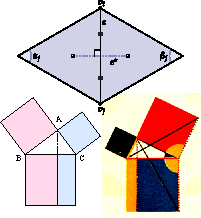
\includegraphics[width=\linewidth]{assets/penrose/EuclideanStyleInspiration.pdf}
   \caption*{Diagrams used as inspiration for the \Style{}s in \cref{fig:ThreeEuclideanStyles}.}
 \end{wrapfigure}


One goal of \Penrose{} is to codify the subjective style choices made by professional illustrators so non-expert users can benefit from their expertise.  \cref{fig:ThreeEuclideanStyles}, \figloc{bottom} cascades on the bare-bones \Style{} program to riff on styles from several existing sources (shown in inset), namely, \emph{Byrne's Euclid}~\cite{Byrne:1847:FSB}, \emph{Wikipedia}~\cite{Wikimedia:2006:IEP}, and a collection of illustrated notes on \emph{discrete differential geometry}~\cite{Crane:2013:DGP}. This figure also illustrates how we can ``mix and match'' different \Style{} and \Substance{} programs. The bulk of these styles (\(\sim\)500 lines) share the same baseline Style code; additional code for a specific style requires less than 100 more lines. To illustrate the Pythagorean theorem (right column), we also used cascading to add diagram-specific features (\eg altitude and extension lines).

\begin{figure}
  \centering

  \begin{minipage}[c]{0.41\columnwidth}  
  \begin{mdframed}[style=SUBCode]
  \begin{lstlisting}[language=Sub-geom,escapechar=@,numbers=none]
Point A, B, C
-- define a right triangle
Triangle ABC := {A,B,C}
Angle $\uptheta$ := $\angle$(C,A,B)
Right($\uptheta$)
-- square each side
Point D, E, F, G, H, I
Square CBDE := [C,B,D,E]
Disjoint(CBDE, ABC)
Square BAGF := [B,A,G,F]
Disjoint(BAGF, ABC)
Square ACIH := [A,C,I,H]
Disjoint(ACIH, ABC
-- split hypotenuse area
Segment AK := Altitude(ABC,$\uptheta$)
Point K := Endpoint(AK)
Segment DE := {D,E}
Point L
On(L, DE)
Segment KL := {K,L}
Perpendicular(KL, DE)
Rectangle BDLK := {B,D,L,K}
Rectangle CKLE := {C,K,L,E}
-- (plus additional objects
-- from Byrne's diagram)\end{lstlisting}
\end{mdframed}
\end{minipage}\hfill
\begin{minipage}[c]{.58\columnwidth}
  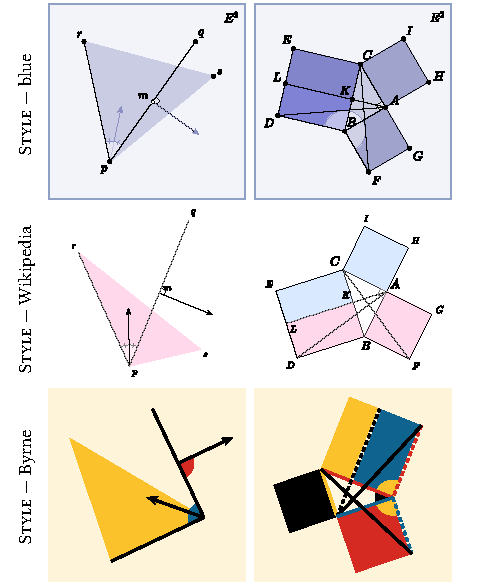
\includegraphics[width=\linewidth]{assets/penrose/ThreeEuclideanStyles.pdf}
\end{minipage}
   \caption{The cascading design of \Style{} enables one to modify a base style with relatively little code.  Here the two \Substance{} programs from \cref{fig:teaser} and the listing above are visualized in three different styles, all of which build on the same basic constraints and objectives.\label{fig:ThreeEuclideanStyles}}\vspace{-\baselineskip}
\end{figure}

In the spirit of Hilbert's quip (\cref{sec:SystemDesign}), we can also swap out the basic visual representation of a given set of logical statements.  For instance, any collection of geometric statements that does not assume the \emph{parallel postulate}  can be realized in several different geometries (\cref{fig:teaser}).  To generate this figure, we wrote three \Style{} programs that all match on the same patterns from a common ``neutral geometry'' \Domain{} schema.  Swapping out these \Style{} files then allows users to build intuition about spherical or hyperbolic geometry by exploring how a given figure (expressed via \Substance{}) differs from its Euclidean counterpart.  Such an example could be further enriched by writing styles for different models of hyperbolic geometry (such as half-plane, hyperboloid, or Beltrami-Klein), each of which involves meticulous calculations.  

% To show that these examples were not cherry-picked, \cref{fig:GeometrySamples} depicts a gallery of samples.

Finally, the diagram specification enables us to build ``staged'' diagrams, such as ones illustrating the steps of a proof.  \cref{fig:byrne-stages} successively uncomments lines of \Substance{} code to produce a style of explanation common in textbooks and slides, a strategy which could easily be applied to (say) any two-column proof. In this example, the values of optimized variables are fixed by hand; an interesting question is how this might be done automatically.

% TODO include a Style listing for the three Style programs in the supplemental material?
% TODO: Compare the code and resulting images to a diagram made in other geometry libraries?


\begin{figure}[t]
   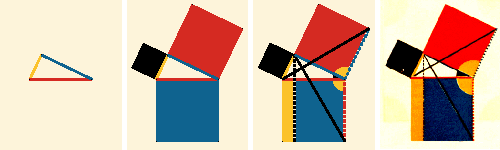
\includegraphics[width=\columnwidth]{assets/penrose/byrne-stages.pdf}
   \caption{Once a complex diagram has been built, it can be easily broken into pieces or stages by, \eg commenting out lines of \Substance{} code.  Here we illustrate steps in Euclid's proof of the Pythagorean theorem, turning Byrne's static figure \figloc{(far right)} into a progressive ``comic strip.''\label{fig:byrne-stages}}
 \end{figure}
 

\subsection{Linear Algebra}
\label{sec:LinearAlgebra}

% (Should we say that doing this creates new capabilities?)
% The difference in \Substance{} is that strings are written by a programmer to convey a mathematical meaning, not automatically generated by production rules.

In mathematics, complexity is built up by composing simple statements. The mapping defined by a \Style{} program automatically lifts this \emph{compositionality} to the visual setting. That is, it enables \Substance\ writers to compose logical statements to build up visual complexity without explicit effort from the \Style{} programmer.  A good analogy is procedural \emph{L-systems}~\cite{Prusinkiewicz:2012:ABP}. Although a graphics programmer can directly write code to recursively apply spatial transformations, it saves effort to first generate strings in a grammar, then systematically translate these strings into graphical transformations.

In \Penrose{}, examples from linear algebra demonstrate compositionality.  The \Style{} declaration on \cref{lin:VectorIsALittleArrowEnd} of \cref{fig:style_linalg} defines the visual icon for a vector (a 2D arrow).  Suppose we now want to illustrate \emph{linear maps}, denoted by \(f\), which have two defining properties: linearity of vector addition (\(f(u+v) = f(u)+f(v)\) for all vectors \(u,v\)) and homogeneity of scalar multiplication (\(f(cu) = cf(u)\) for all vectors \(u\) and scalars \(c\)).  Successive \Style\ rules cascade on \cref{fig:style_linalg} to define how these logical operations  should be mapped to visual transformations.  For example, application of a linear map \(f\) is represented by a literal $2 \times 2$ matrix-vector multiply; the image vector \(f(u)\) also inherits the color of the argument \(u\). The map itself is visually represented by a labeled arrow, and the domain and target spaces by coordinate planes on either side. The \Style{} programmer need not compose these directives explicitly; the compiler does the tedious job of translating \Substance{} statements (\cref{fig:linearMap}, \figloc{top}) into a composition of graphical statements that define a diagram (\cref{fig:linearMap}, \figloc{bottom}).  Moreover, since the \Style{} program faithfully represents the underlying mathematics, we observe the expected properties, \eg the arrow for \(f(u_1+u_2)\) is the same as the arrow for \(f(u_1)+f(u_2)\).  Automatically checking consistency of the visual representation based on analysis of a richer \Domain{} schema would be an interesting topic for future work.

% (addition, scaling, and application of linear maps)
% \setlength{\columnsep}{1em}
% \setlength{\intextsep}{0em}
% \begin{figure}{l}{140pt}
\begin{center}
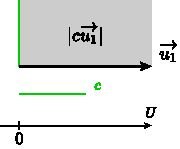
\includegraphics[width=140pt]{assets/penrose/LinearAlgebra1D.pdf}
\end{center}
% \end{wrapfigure}

Finally, the inset (above) shows an alternative representation for vectors and scalars as signed and unsigned quantities ($u_1$ and $c$, \resp{}) on the number line.  The benefit of a 1D representation is that the remaining dimension can be used to illustrate different concepts, in this case relating the magnitude of a product to an area.  The ability to switch between representations can be pedagogically valuable, such as for transitioning from lower to higher mathematics.

\begin{figure}
  \begin{minipage}[t]{0.45\columnwidth}
   \begin{mdframed}[style=SUBCode]
    \begin{lstlisting}[language=Sub-LA,escapechar=@,numbers=none]
VectorSpace U, V
LinearMap f : U $\rightarrow$ V
Vector u1, u2, u3 $\in$ U
Vector v1, v2, v3, v4 $\in$ V
u3 := u1 + u2
v1 := f(u1)
v2 := f(u2)
v3 := f(u3)
v4 := v1 + v2
\end{lstlisting}
   \end{mdframed}
\end{minipage}\hfill
  \begin{minipage}[t]{0.45\columnwidth}
   \begin{mdframed}[style=SUBCode]
    \begin{lstlisting}[language=Sub-LA,escapechar=@,numbers=none]
VectorSpace U, V
LinearMap f : U $\rightarrow$ V
Vector u1, u2 $\in$ U
Vector v1, v2, v3 $\in$ V
Scalar c
u2 := c * u1
v1 := f(u1)
v2 := f(u2)
v3 := c * v1 \end{lstlisting}
   \end{mdframed}
  \end{minipage}
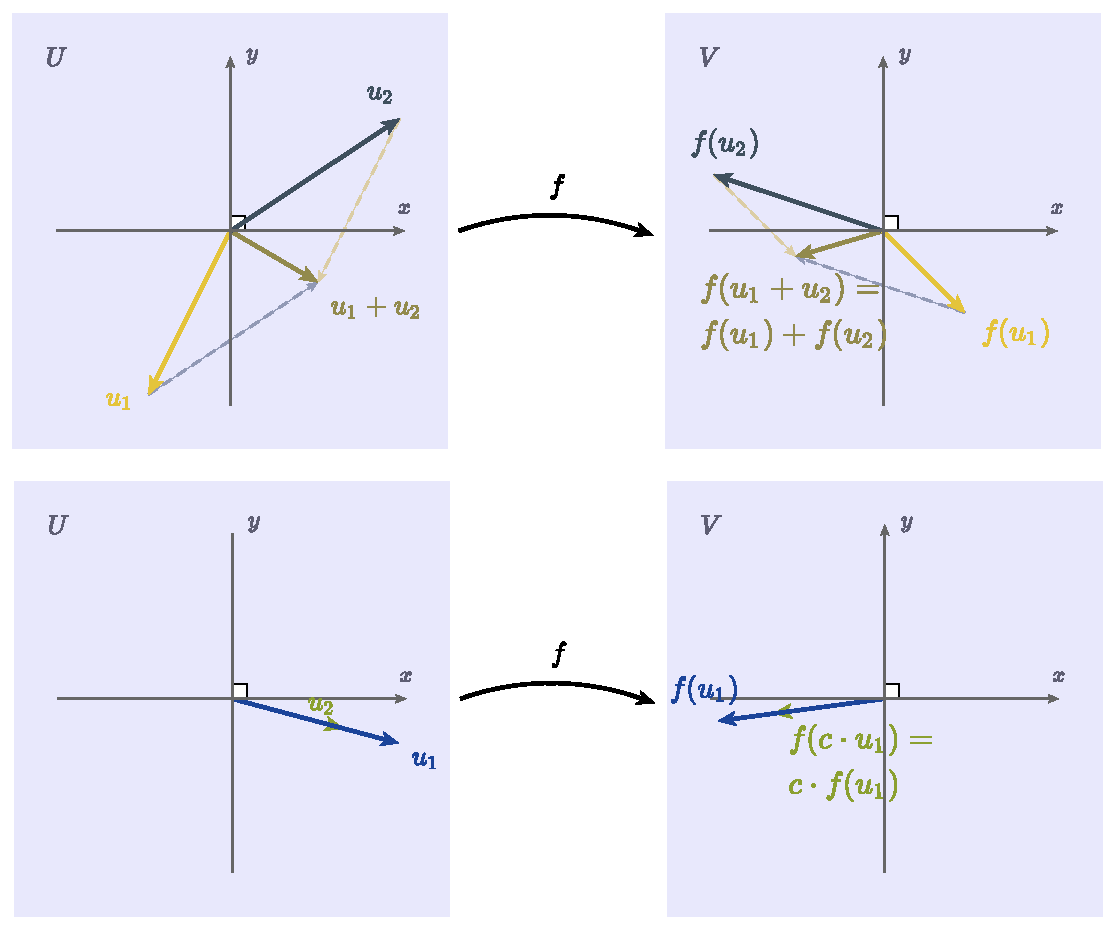
\includegraphics[width=\columnwidth]{assets/penrose/linearmap-add-scale.pdf}
   \caption{Composition of mathematical statements naturally translates into composition of graphical transformations with no explicit programmer effort.  Here we compose linear maps, showing addition and scaling, to illustrate the two defining properties of linear maps.\label{fig:linearMap}}
\end{figure}


% AutoLabel All
% Label u1 $u_1$
% Label u2 $u_2$
% Label u3 $u_1 + u_2$
% Label v1 $f(u_1)$
% Label v2 $f(u_2)$
% Label v3 $f(u_1 + u_2) = \\ f(u_1) + f(u_2)$
  
% \todo{Fix the label strings above so they aren't typeset?}

% AutoLabel All
% Label u1 $u_1$
% Label u2 $u_2$
% Label v1 $f(u_1)$
% Label v2 $f(c \cdot u_1) = \\ c \cdot f(u_1)$
% Label v3 $f(c \cdot u_1) = \\ c \cdot f(u_1)$      

%   \begin{overpic}[scale=0.4]{assets/penrose/linalg-vectorsadd3.pdf}
%     \put(2,80) {\parbox{2in}{
%         \texttt{\textbf{VectorSpace} U} \\
%         \texttt{\textbf{Vector} u1, u2, u3,} \\
%         \texttt{\mbox{              } u4, u5} \\
%         \texttt{u3 := u1 + u2} \\
%         \texttt{u5 := u3 + u4}
%         }}
%     \end{overpic}
% \caption{A simple \Substance{} program that specifies that several vectors are added results in a gallery of diagrams illustrating the given relationships. \label{fig:PenroseWorkingLA}}

\begin{figure}
\begin{mdframed}[style=SUBCode]
\begin{minipage}[t]{.47\columnwidth}
\begin{lstlisting}[language=Sub-mesh,escapechar=@,numbers=none]
SimplicialComplex K
Edge e $\in$ K
Subcomplex E $\subseteq$ K
E := Closure(e)
SimplicialSet StE $\subseteq$ K
StE := Star(E)
Subcomplex ClStE $\subseteq$ K
\end{lstlisting}
\end{minipage}
\ContinueLineNumber
\begin{minipage}[t]{.5\columnwidth}
\begin{lstlisting}[language=Sub-mesh,escapechar=@,numbers=none]
ClStE := Closure(StE)
Subcomplex ClE $\subseteq$ K
ClE := Closure(E)
SimplicialSet StClE $\subseteq$ K
StClE := Star(ClE)
SimplicialSet LkE $\subseteq$ K
LkE := SetMinus(ClStE, StClE)\end{lstlisting}
\end{minipage}
\end{mdframed}
   \centering
   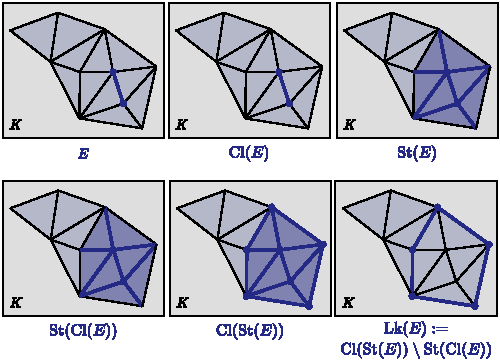
\includegraphics{assets/penrose/mesh-figure.pdf}
   \caption{A language-based specification makes it easy to visually inspect data structures or assemble progressive diagrams with only minor changes to program code.  Here we draw the simplicial \emph{link} by building it up from simpler constituent operations.\label{fig:substance-mesh-clst}}
\end{figure}

\begin{figure}
   \centering
   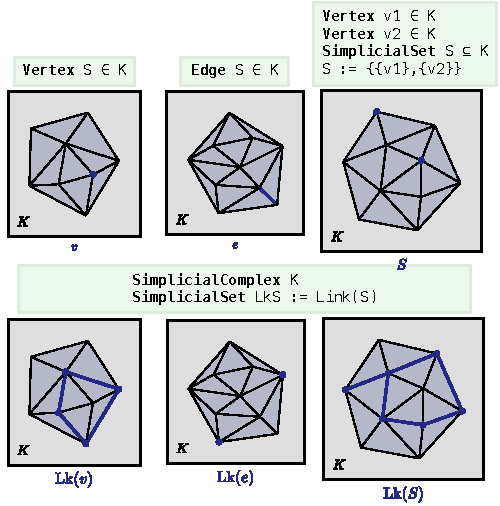
\includegraphics[scale=1.5]{assets/penrose/mesh-examples.pdf}
   \caption{Domain-specific notation makes it easy to explore an idea by trying out many different examples.  Here several subsets of a simplicial complex are specified \figloc{(top)} to explore the definition of the ``link'' \figloc{(bottom}).  An external plugin generates random example meshes, further enriching exploration.\label{fig:mesh-examples}}
\end{figure}

\subsection{Meshes}
\label{sec:Meshes}

Polygonal meshes are ubiquitous in computer graphics, but illustrating meshes is often cumbersome due to the large number of elements involved, especially when illustrating meshes by hand or in GUI-based tools.  In such cases, \Penrose{} can be useful not just for making illustrations, but also to inspect and debug user-defined data structures by attaching them to custom visualizations.  A simple example is shown in \cref{fig:substance-mesh-clst}, where different regions of a mesh are specified via standard operators on a simplicial complex; this diagram also illustrates the definition of the simplicial \emph{link}~\cite[Section 3.3]{Bloch:1997:FCG}.  Further examples in \cref{fig:mesh-examples} show how a user can quickly build intuition about this definition by drawing the link of a variety of different mesh subsets.

To make these examples in \Penrose{}, we follow a pattern similar to the discrete function example (\cref{sec:Functions}): generic mesh objects from the \Substance{} code are refined into specific instances of \inlineSUB{\keyword{Vertex}}, \inlineSUB{\keyword{Edge}}, and \inlineSUB{\keyword{Face}} objects by an external plugin, which generates and optimizes a random triangle mesh.  Since meshes are randomly generated, the plugin passes a random seed (from its \Style{} arguments) to draw different pieces of the same mesh.  For this example, we used an existing JavaScript-based mesh processing library~\cite{Sawhney:2017:GPJ} that was not designed ahead of time to interface with \Penrose{}.  The benefit of generating these elements at the \Substance{} level (rather than returning, say, a static SVG image) is that they can continue to be styled and manipulated within \Penrose{}; the programmer does not have to edit extra graphics code or keep it compatible with the \Style{} program.  Likewise, programmers who adopt \Penrose{} as a tool for visual debugging can benefit from system improvements while writing minimal code to attach their data structures to a visual representation.

% AutoLabel E
% AutoLabel e
% AutoLabel K
% Label S1 $\mathrm{St}(E)$
% Label A $\mathrm{Cl}(\mathrm{St}(E))$
% Label B $\mathrm{Cl}(E)$
% Label S2 $\mathrm{St}(\mathrm{Cl}(E))$
% Label S3 $\mathrm{Lk}(E) := \mathrm{Cl}(\mathrm{St}(E)) \setminus \mathrm{St}(\mathrm{Cl}(E))$
% Label S4 $\mathrm{Lk}(E)$
% SimplicialSet S4 $\subseteq$ K
% S4 := Link(E)

% Result(E) -- Cl(e)
% Result(B) -- Cl(E)
% Result(S1) -- Star(E)
% Result(A) -- Cl(S1)
% Result(S2) -- St(B)
% Result(S4) -- Lk(E)

%%%%%%%%%%

% SimplicialComplex K
% Vertex v1 $\in$ K
% Vertex v2 $\in$ K
% SimplicialSet S $\subseteq$ K
% S := Union(v1, v2)
% SimplicialSet S1 $\subseteq$ K
% S1 := Link(S)
% Result(S1)
     
\subsection{Ray Tracing}
\label{sec:RayTracing}

\begin{figure}
   % PathType t1, t2, t3
   % HasForm (t1, "L(D|S)SE")
   % HasForm (t2, "LSDE")
   % HasForm (t3, "LE")

   % Path p1, p2, p3
   % p1 := Sample(t1)
   % p2 := Sample(t2)
   % p3 := Sample(t3)
   \centering
   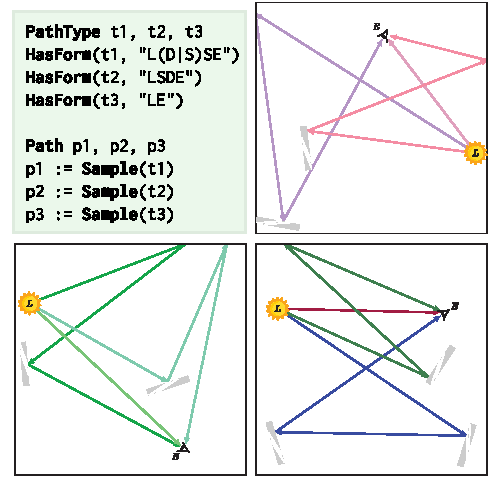
\includegraphics[scale=1.5]{assets/penrose/rt-multiple-paths.pdf}
   \caption{When drawing ray tracing diagrams by hand, it can be difficult to construct geometry that permits the desired path types.  Here we jointly optimize path and scene geometry to match multiple path types simultaneously.  Shown are several diagrams generated for the same program.\label{fig:rt-multiple-paths}}
\end{figure}


Our final example constructs light path diagrams, which are often used to illustrate ideas in physically-based rendering.  The \Substance{} code expresses types of light paths via Heckbert's regular expression notation.  For instance, the expression \inlineSUB{\texttt{L(D|S)S*E}} specifies a family of light paths that start at a light source (\inlineSUB{\texttt{L}}), bounce off a diffuse or specular object (\inlineSUB{\texttt{S|D}}), then bounce off zero or more specular objects (\inlineSUB{\texttt{S*}}), then enter the ``eye'' or camera (\inlineSUB{\texttt{E}}).  One or more paths can then be declared that have a given form (\cref{fig:rt-multiple-paths}).  The challenge in generating a diagram from such a specification is that there must be geometry in the scene that supports the given path(s).  For instance, for a fixed eye, light, and mirror, there may simply be no path of the form \texttt{LSE}.  Rather than meticulously constructing a valid scene by hand, we can use a simple \Style{} program to jointly optimize the scene geometry and the light path by specifying constraints such as equality of incoming and outgoing angles at a specular bounce.  The set of objects in the scene is generated by a simple plugin that expands the regular expression into a set of compatible objects (\eg a mirror for each specular bounce).  This plugin also uses the canvas size to choose appropriate scene and path complexity according to the target output device (\cref{fig:Retargeting}).  Diagrams for more intricate light transport phenomena could be generated by calling an actual ray tracer (such as \emph{PBRT}~\cite{Pharr:2016:PBR}) to trace and rejection-sample paths by path type.  The added value of generating the final diagrams with \Penrose{} is that initial path and scene geometry generated by the external code can be further optimized to meet other design goals, such as the canvas size. Additionally, the visual style of a large collection of diagrams (\eg for a set of course notes) can easily be adjusted after the fact.

In our experience, \Penrose{} acts as a \emph{nexus} for diagram generation. It connects disparate components, such as language-based specification and ray tracing, into a diagramming tool that provides the system-level benefits described in \cref{sec:Introduction}.



% This is the selector for positioning the mirror for a specular bounce, which is interesting but too long/involved to include

% PathEdge e1; PathEdge e2; Path ps
% where e1 := CreateEdge(v1, v2);
%       e2 := CreateEdge(v2, v3);
%       IsSpecular(v2); Hits(v2, o)
% with PathVertex v1, v2, v3; SpecularObject o {
%     LOCAL.mirrorPadding = 1.0
%     LOCAL.horizontalShift = sampleReal(o.shape.w / -2.0 + 20.0, o.shape.w / 2.0 - 20.0)
%     override o.shape.rotation = mirrorAngle(e1.shape, e2.shape)
%     override o.shape.x = mirrorPosX(e1.shape, e2.shape, v2.x, v2.y, o.shape.h / 2.0 + LOCAL.mirrorPadding, LOCAL.horizontalShift)
%     override o.shape.centerY = mirrorPosY(e1.shape, e2.shape, v2.x, v2.y, o.shape.h / 2.0 + LOCAL.mirrorPadding, LOCAL.horizontalShift)
%   }

% \begin{figure}
%   \begin{overpic}[scale=0.15]{assets/penrose/rt-samples.pdf}
%       \put(-5,75) {\parbox{2in}{
%           \texttt{\textbf{PathType} t} \\
%           \texttt{\textbf{HasForm}(t,"L(D|S)S*E")} \\
%           \texttt{\textbf{Path} p := \textbf{Sample}(t)}
%         }}
%     \end{overpic}
%         \caption{ \label{fig:rt-samples}}
% \end{figure}

% \begin{figure}
%   \begin{minipage}[!t]{.4\columnwidth}
%   \begin{lstlisting}[language=Sub-RT,escapechar=@]
% PathType t1, t2, t3
% HasForm(t1, "L(D|S)SE")
% HasForm(t2, "LSDE")
% HasForm(t3, "LE")

% Path p1, p2, p3
% p1 := Sample(t1)
% p2 := Sample(t2)
% p3 := Sample(t3) \end{lstlisting}
% \end{minipage}\begin{minipage}[!t]{.6\columnwidth} 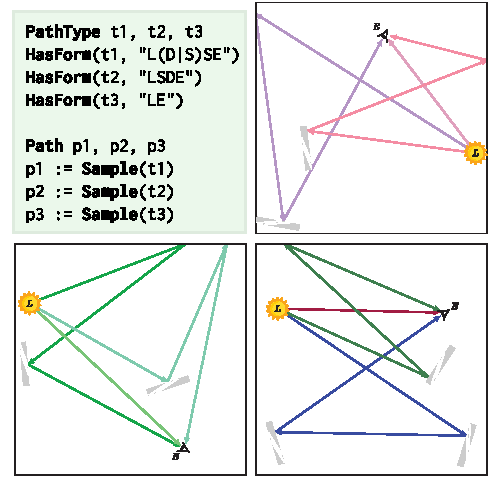
\includegraphics[width=\columnwidth]{assets/penrose/rt-multiple-paths.pdf}
% \end{minipage}
% \caption{When drawing ray tracing diagrams by hand, it can be difficult to construct scene geometry that permits the desired types of paths. With our optimization based layout, objects in the scene can be automatically arranged to satisfy complex path descriptions. Here we show a scene that simultaneously supports several different path types. \label{fig:rt-multiple-paths}}
% \end{figure}

\subsection{Large-Scale Diagram Generation}
\label{sec:LargeScaleDiagramGeneration}

One goal for \Penrose{} is that effort spent on diagramming should be generalizable and reusable (\ref{gol:Reuse}). To demonstrate the system's reuse potential, we developed a simple program synthesizer to automatically create any number of diagrams randomly sampled from a domain. Given a \Domain{} program, a \Style{} program, and the number of diagrams (\textsf{n}) as input, the synthesizer analyzes the \Domain{} program to find the mathematical constructs in the domain, randomly creates \textsf{n} \Substance{} programs that contain these constructs, then compiles, optimizes, and renders the results. \cref{fig:enumerate-subsets} demonstrates an example of using the synthesizer to ``autocomplete'' an underspecified \Substance{} program by automatically enumerating all possible subset relationships, using information from the \Domain\ schema. Automatically generating diagrams at scale can also help users write better \Style{} programs, since synthesizer can ``fuzz'' the space of possible \Substance{} programs to find corner cases.

To stress-test the system's performance and the reusability of \Style{} and \Domain{}\ programs, we randomly generated 2000 \Substance{} programs from the sets domain (\cref{sec:Sets}) in the flat disc style. \Penrose{} was able to create diagrams for all samples. Though 1058 of the 2000 programs had conflicting constraints due to randomness, the solver failed gracefully (as in \cref{fig:sets-inconsistent}) and reached convergence.

\subsection{Performance Evaluation}
\label{sec:PerformanceEvaluation}

We hope to support an iterative workflow where the system's performance does not block the user's creative process. One possible goal is to generate most diagrams within ten seconds, since that threshold is deemed a ``unit task'' in cognitive science~\cite{unifiedTheoriesCognition} and is about as long as similar authoring processes take, such as building a \LaTeX{} document or compiling code. Even lower latency ($<$ 500 ms) might enable new applications of \Penrose, since this threshold benefits users of data visualization, live programming, and other exploratory creative tools~\cite{Liu:latency:2014}.

\begin{figure}
  \centering
  \includegraphics[width=.7\columnwidth]{assets/penrose/optimization-graph.pdf}
  \caption{To stress-test the system and collect timing information, we generated and visualized random \Substance\ programs of different sizes, revealing that optimization dominates the execution time.
    \label{fig:optimization-performance}
  }
\end{figure}

\begin{figure}
  \centering
  \includegraphics[width=.7\columnwidth]{assets/penrose/compilation-graph.pdf}
  \caption{We evaluated the performance of the \Penrose{} compiler by running it on a large collection of programs, showing that the execution time of the compiler grows slowly as the number of selector matches increases.
    \label{fig:compilation-performance}
  }
\end{figure}

We have not focused on performance tuning, so a fully-interactive experience is not yet possible with \Penrose{}. With our current na\"ive implementation, \Penrose{} generated 70\% of the figures in this chapter in under 10 seconds. However, some figures took significantly longer (\eg{} \cref{fig:teaser}, \cref{fig:DomainInterop}, and \cref{fig:ThreeEuclideanStyles}), up to a few minutes. To assess the system's performance, we used diagrams generated in \cref{sec:LargeScaleDiagramGeneration} to simulate arbitrary user inputs and measured the time to produce each diagram. To analyze the relative performance of different parts of the system, we separately timed the four stages in the layout engine (\cref{sec:LayoutEngine}): compilation, optimization, label generation, and rendering.  Timing was measured on a 2017 MacBook Pro; note that performance in our web-based IDE (\cref{sec:DevelopmentEnvironment}) is slower due to the cost of editor services and communication with the browser.  As shown in \cref{fig:optimization-performance}, optimization dominates execution time, though the time to convergence grows slowly with the size of the optimization problem. The second slowest part is the compiler, though \cref{fig:compilation-performance} shows that compilation time grows linearly with the number of selector matches, suggesting that the compiler scales well.

We are optimistic about our ability to improve the optimization speed, since we are currently using only a simple, generic solver that we implemented ourselves. (See \cref{sec:Solver} and \cref{sec:DiscussionandFutureWork} for further discussion.) In our experience, optimization often slowed by objectives that involve all pairs of a large collection of objects, especially for label placement, where all labels ``repel'' all others.  Here one could apply standard acceleration strategies for \(n\)-body problems, such as the Barnes-Hut algorithm~\cite{Barnes:1986:barneshut}.  Moreover, though it may take time for diagrams to finish, the optimization-based approach provides near-instantaneous \emph{feedback} for most diagrams by displaying the first few steps of the optimization process.  These proto-diagrams typically provide enough information about the final layout that the user can halt optimization and continue iterating on the design.

% Finally, temporarily disabling certain diagram elements (such as labels) accelerates the iteration process.

% However, we hope to continue improving interactivity via further optimization of the compiler and layout engine, as well as using the constraint-based specification to precompute interactive experiences (in the spirit of tools like \emph{GeoGebra}).

% \section{Related Work}
% \label{sec:RelatedWork}

% Q: Why not just defer our entire related work section to the CHI paper?
% A: Because the one and only aim of the related work section should be comparing/contrasting our approach to existing approaches, or pointing out explicitly how our system builds on ideas from previous tools.

% It should not be a survey or taxonomy of diagramming tools (as it may have appropriately been in the CHI paper).
% So, the way to write it is to ask in each sentence:
% What can I say about this tool/category of tools in relation to our system design?
% What specific subsections or figures can I point to when mentioning this tool?
% If there is no such connection, you can likely omit it.

% Anyway, that should make for a very different section than the CHI paper.

% The mappings can be applied in a variety of ways to obtain new capabilities that are difficult to achieve using existing tools (\cref{sec:RelatedWork}).

% The categories in the ICERM talk were:
% GUI, low-level languages, specialized packages, plotting software

% Do language workbenches count?
% Should we cite only things that haven't been cited yet?

% General diagramming tool (non-specialized): Illustrator, Keynote, etc.
% Visualizing mathematics through plotting: Mathematica, matplotlib, D3, etc.

%%%%%%%%%%%%%%%%%%%%%%%%%%%

% Language as an input: Mathematica, Geogebra, TikZ, GCLC, xy-pic, graphviz, also specialized tools.

% Separation of content and style (or, similarly, encoding a formal mapping from content to style): CSS, Grammar of graphics, Vega-Lite.

% Automatic optimization/constraint-based layout: Sketchpad, GCLC, Basalt, g9.js, etc.

% Specialized software for visualizing logical relationships in one domain: Group Explorer, euclid.js, chemical diagram software, Mermaid, UML diagrams,etc.


\section{Discussion and Future Work}
\label{sec:DiscussionandFutureWork}

% Examples of good conclusions:
% http://people.csail.mit.edu/jrk/halide12/halide12.pdf
% http://graphics.stanford.edu/papers/scanner/poms18_scanner.pdf

% Characterize the problem and needs
% Say why the problem is hard
% Characterize the state of the art
% Say what we did and why it matters, in terms of tackling the larger problem
% Say the implications of our work
% Say what is left to tackle the larger problem, and what new problems or lines of inquiry our work opens up

% Now that we (as readers, and as system builders) understand the problem and a proposed solution more deeply, what new things are we able to say about it that we couldn't before??

% \todo{} diagrams that help to spark/inspire thoughts about future work, but don't have to have completely automated/general solutions).

% Although we focused in this paper on this specific stuff, the principles we use can lead to much more
% (We have lots of future work that we haven’t gotten to)
% Fill the section w/ all the cool stuff we want to do
% Point out why the system can make this stuff possible

% Talk about the limitations…. every limitation is an opportunity for future work
% Limitations and future work
% Here’s a limitation. But note that X. In the future, we hope to X.
% Go to #issues and look for tags #open-ended and #feature-request

% TODO: One big question is going to be: Are people using Penrose? Has the system proven itself useful in that way? Not sure how (or if) to address that.

% TODO: are there any other cross-cutting concerns to discuss?

% Improving web presentation capabilities was a topic of interest to many in the web community and nine different style sheet languages were proposed on the www-style mailing list.[25] Of these nine proposals, two were especially influential on what became CSS: Cascading HTML Style Sheets[21] and Stream-based Style Sheet Proposal (SSP).
% https://en.wikipedia.org/wiki/Cascading_Style_Sheets#History

% problem, motivation, initial step, future work (in one par)

% It's still hard to communicate mathematics visually. However, it is obviously still important.
% In a way that codifies the best practices of mathematical illustrators into a format that is reusable and broadly accessible. Much like TeX.
% opening the way toward many capabilities that aren't enabled by existing diagramming tools.
% These representations should afford XX...
% How to talk about this without just summarizing what a PL is?
% It's possible that the right levels of abstraction, the interfaces between layers of the system, and ways of expressing the ideas haven't been designed.
% However, we think our system offers some concrete suggestions in this direction.

Effectively communicating mathematical ideas remains a major challenge for students, educators, and researchers alike. \Penrose\ provides a step toward understanding the abstractions needed to build general-purpose diagramming tools that connect a concise specification of mathematical content with powerful tools for visual synthesis.  In our experience, centering the design around \emph{mappings} from logical to visual objects leads to a system that is both flexible and scalable.  Moreover, providing a clean separation between content and presentation lays a foundation for meaningful interaction techniques for making diagrams.

The system has several limitations that make interesting topics for future work. For example, the \Domain, \Substance, and \Style\ languages are limited in what they can express. Thus, \Substance\ might be extended with more constructs from mathematical language, such as anonymous expressions, and \Style\ might be extended to provide greater flexibility, \eg{}, via user-defined priorities on objectives. Additionally, the system currently supports only a fixed set of objectives, constraints, functions, graphical primitives, and renderers, as detailed in~\cref{sec:Implementation}. However, our software architecture does not present major roadblocks to greater extensibility, such as enabling programmers to define constraints inline or emit output for other targets such as 3D or interactive platforms. The system also presents opportunities to study questions of usability, learnability, and debugging, such as the natural way that \Style\ users might want to express spatial layout constraints and the learning curve for different classes of users. 

The cost of optimization is the biggest bottleneck in our pipeline, as seen in \cref{sec:PerformanceEvaluation}, which is not surprising given that we currently use a ``catch-all'' solver.  A nice feature of our design is that the program semantics provide rich information about the structure of the optimization problem.  This structure should make it possible to adopt highly effective problem-specific optimization strategies of the kind described in \cref{sec:OptimizationBasedSynthesis} and \cref{sec:PerformanceEvaluation}, \eg{} analyzing the computation graph to break down the diagram into smaller constituent pieces.  Beyond finding local minima, we are excited about different design modalities enabled by exploring the constraint space defined by the \Style{} program, such as sampling a diverse set of examples or interpolating between different layouts to create animations.

Finally, there is no reason that the basic design of \Penrose{} must be applied only to mathematical diagrams. Many other fields, such as law, chemistry, and biology, all deal with non-quantitative information comprised of intricate logical relationships.  We believe that an extensible and expressive system for assigning visual interpretations to such information provides a powerful tool for seeing the big picture.

% Currently, for instance, objectives and constraints must be added by the user at the system level, rather than to individual \Style{} programs. 
% Likewise, the system assumes a particular rendering frontend (currently 2D vector graphics).
% Another direction for future work is to make it easier for users to extend the capabilities of the system itself, for example by extending the standard library of objectives, constraints, functions, graphical primitives, plugins, and renderers.

% primitives for iteration, 
% encoding a more diverse set of domains in \Penrose\ might be explored by systematically sampling and implementing a set of domains from the Mathematics Subject Classification Scheme, a classification scheme used to categorize mathematical journal articles~\cite{mathsubject:rusin}.
% How difficult is it for domain novices, domain experts, and diagramming experts to pick up Penrose? How can the design of \Penrose\ be strengthened to support the process of creative iteration? 
% One might design user studies following the ``natural-programming'' approach~\cite{myers2004natural} to investigate any of these questions. 
 
% Removed for double-blind
% \section{Acknowledgments}


% --------------------------------------------------------------------------------

% In \Penrose{}, a low-level API does exist, though only internally, as a means to implementing the compiler (\cref{sec:Compiler}), though in principle could be exposed to the user if they wanted to do crazy stuff.

% 1. API
%     - PROS:
%     - CONS:
% 2. Visual programming language
%     - PROS:
%     - CONS:
% 3. (Conventional) programming language
%     - PROS:
%     - CONS:



% Our first design decision is to \textbf{use \textit{language} to codify the relationship between abstract concepts and their visual representations.} Language is a concise way to represent shared knowledge. From there, is is natural to split it into a language for expressing logical relationships, another language for expressing visual representations of those relationships, and a language to express what logical relationships are possible. As a secondary design decision, and a cross-cutting systems issue, our language design is organized around the use of \textit{types} that serve different purposes in each language: modeling logical relationships, declaring objects, and matching styles to objects. Two alternatives to language that we considered were a GUI or an API, but a language seemed more general than both of them, so we picked the more fundamental solution.


% \setlength{\columnsep}{1em}
% \setlength{\intextsep}{0em}
% \begin{wrapfigure}{r}{.45\textwidth}
% \vspace{-10pt}
%   \begin{center}
%     \includegraphics[width=0.45\textwidth]{assets/chapter-2/penrose-trio.pdf}
%   \end{center}
% \end{wrapfigure}

% Instead of a limited focus on one specific domain (as in GraphViz~\cite{graphviz} for graph theory or GroupExplorer~\footnote{\url{https://github.com/nathancarter/group-explorer}} for group theory), \Penrose is extensible to user-defined domains of diagramming. Both \Substance and \Style are parametrized by a \colorbox[HTML]{DBDBDB}{\Domain} schema that defines all possible objects (\eg \sub{Set}) and relations (\eg \sub{IsSubset}) in a particular domain, which can be used by associated \Substance and \Style programs. In addition to user-extensibility, a formally encoded domain also enables automatic generation of \Penrose diagrams. 

% \Penrose compiles a \textbf{trio} of \Domain, \Substance, and \Style into a constrained optimization problem defined by a set of graphical constraints (\eg arrows that represent vectors should start from the origin). The optimization problem is in standard form, \ie, minimization of an objective function subject to equality and inequality constraints~\cite{convexOptimization}. Such problems may be solved with many standard methods. \Penrose currently uses an exterior point method~\cite{exteriorPoint} that starts with an infeasible point and pushes it toward a feasible configuration via progressively stiffer penalty functions---mirroring a process often used by hand.

% The design of \Penrose is driven by the design goals of reuse and scalability, and therefore is suitable for large-scale generation of visual content. The system is scalable and reusable in several dimensions:
    
% % \setlength{\columnsep}{1em}
% % \setlength{\intextsep}{0em}
% % \begin{wrapfigure}{r}{.45\textwidth}
% % \vspace{-10pt}
% %   \begin{center}
% %     \includegraphics[width=0.45\textwidth]{assets/chapter-2/func-continuous-discrete-vert.pdf}
% %   \end{center}
% % \end{wrapfigure}

% \vspace{1em}
% \begin{figure}[h]
% \begin{minipage}[b]{0.48\linewidth}
% $\bullet$ The optimization problem produced by \Penrose often has multiple solutions, and each point in the solution space corresponds to an alternative diagram. No program changes are required to generate these alternatives.
%     \vspace{3pt}

% $\bullet$ For a visual representation encoded by a \Style program, a wide range of notations (\ie, \Substance programs) can be visualized without any changes to \Style. In the figure on the left, a single discrete \Style program is used to visualize three \Substance programs that describe injective, surjective, and bijective functions.
%     \vspace{3pt}

% $\bullet$ Conversely, multiple \Style{} programs can be applied to the same \Substance{} program, generating alternative visual representations of the same underlying entities. The \Substance programs in the figure are also visualized by an alternative continuous \Style.
% \end{minipage}
% \hfill
% \begin{minipage}[b]{0.5\linewidth}
%     \centering
%     \includegraphics[width=\textwidth]{assets/chapter-2/injection-surjection-bijection.pdf}
% \end{minipage}
% \end{figure}
    
% With the extensible design, \Penrose can automatically generate diagrams from many different domains using familiar syntax. \Penrose-generated geometry, real analysis, ray-tracing, set theory, and algebra are shown below.

% \vspace{10pt}
% \includegraphics[width=0.95\linewidth]{assets/chapter-2/gallery.pdf}